\documentclass{beamer}
%\usepackage{beamerarticle}
\usepackage{heppennames}
\usepackage{hepnicenames}
\usepackage{graphicx} 
\usepackage{multirow}
\usepackage{amsbsy,amsmath,amssymb}
\usepackage{booktabs}
% ********** Styl prezentacji **********
\mode<presentation>
{
	\usetheme{Singapore}
  \setbeamercovered{transparent}
   \setbeamertemplate{footline}[frame number] 
  \setbeamertemplate{navigation symbols}{ 
  \insertslidenavigationsymbol
  \insertframenavigationsymbol
  \insertsubsectionnavigationsymbol
  \insertsectionnavigationsymbol
  \insertdocnavigationsymbol
  \insertbackfindforwardnavigationsymbol
  \hskip 0.3cm
  %\insertframenumber / \inserttotalframenumber  % <<< frame #
  %\insertpagenumber / \insertpresentationendpage % <<< page #
} 
}

\usepackage[english]{babel}
\usepackage[latin1]{inputenc}

% font definitions, try \usepackage{ae} instead of the following
% three lines if you don't like this look
\usepackage{mathptmx}
\usepackage[scaled=.90]{helvet}
\usepackage{courier}


\usepackage[T1]{fontenc}

\author{S. Poss for the CERN LCD group}
\institute[CERN]{CERN}

\subject{CLICCDR}
\AtBeginSection[]
{
	\begin{frame}<beamer>
		\frametitle{Outline}
		\tableofcontents[currentsection,currentsubsection]
	\end{frame}
}

\title[]{CLIC Physics CDR}
%%\subtitle{Our experience}

\date{\today}

\begin{document}

\begin{frame}
	\titlepage
\end{frame}

\begin{frame}
\frametitle{Outline}
\tableofcontents
% You might wish to add the option [pausesections]
\end{frame}


\section{Physics Motivations}
\begin{frame}
\frametitle{Physics Motivations}
\begin{columns}[c]
\column{6cm}
\begin{itemize} 
  \item \alert{Precision measurements} of new particles discovered at the LHC:
  Higgs, SUSY,\ldots\\
  ~\\ 
  \item \alert{Discovery} of new physics at TeV scale
\end{itemize}
\column{6cm}
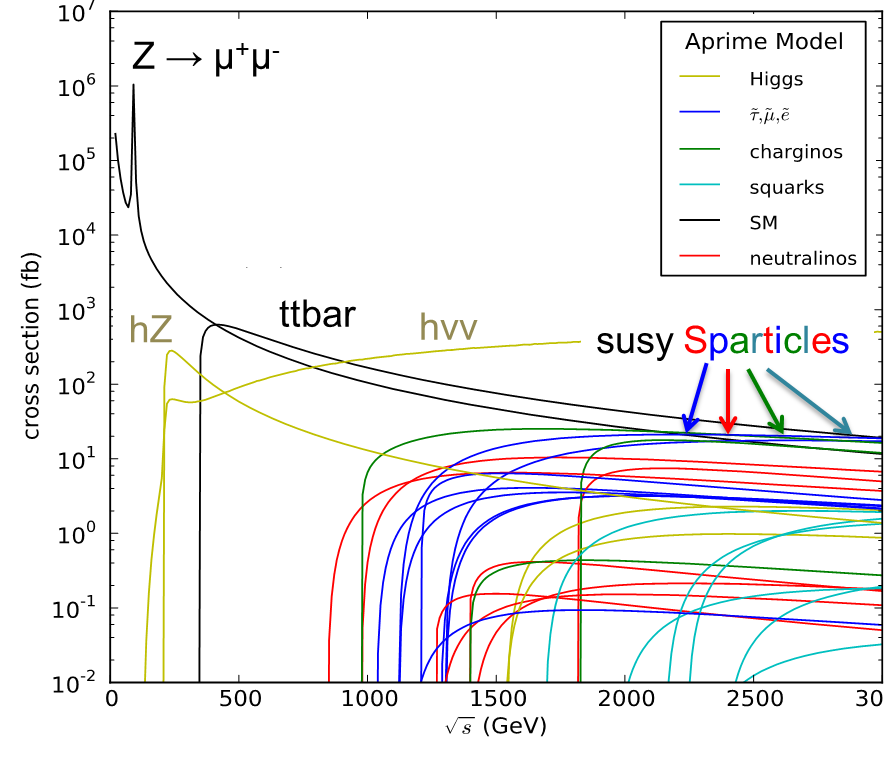
\includegraphics[width=6cm]{models}
\end{columns}
\end{frame}

\begin{frame}
\frametitle{Higgs measurements}
\centering
\begin{columns}[c]
\column{6cm}
\centering
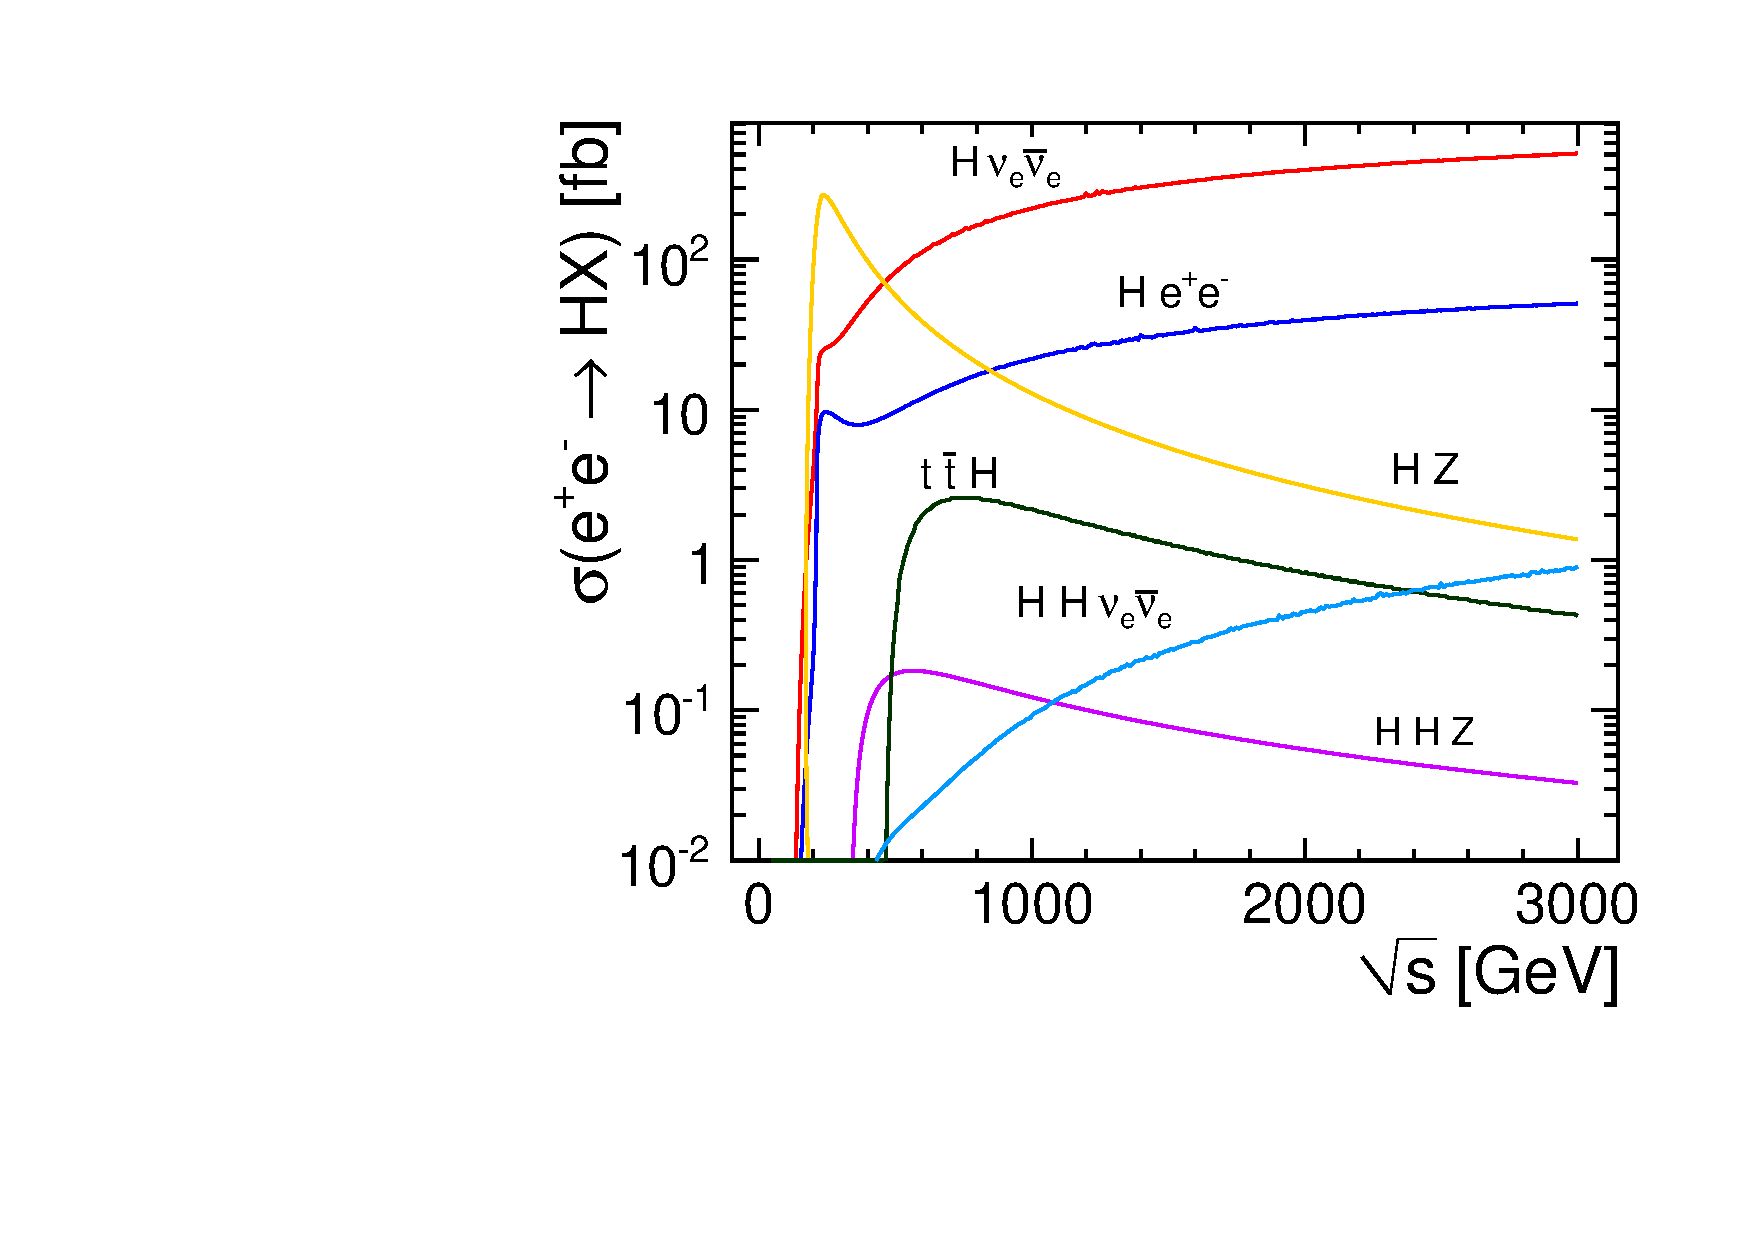
\includegraphics[width=4cm]{xsec_vs_cme}
\column{6cm}
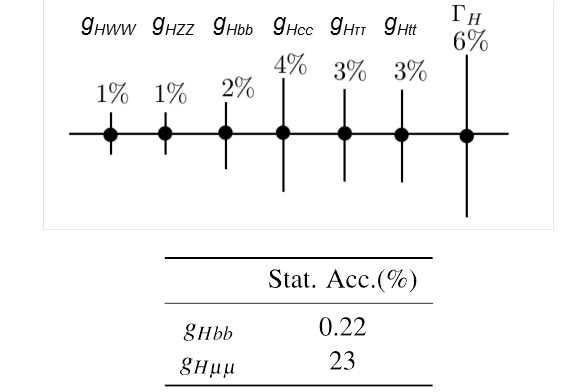
\includegraphics[width=3cm]{higgs}
\end{columns}
\begin{columns}[c]
\column{6cm}
\centering
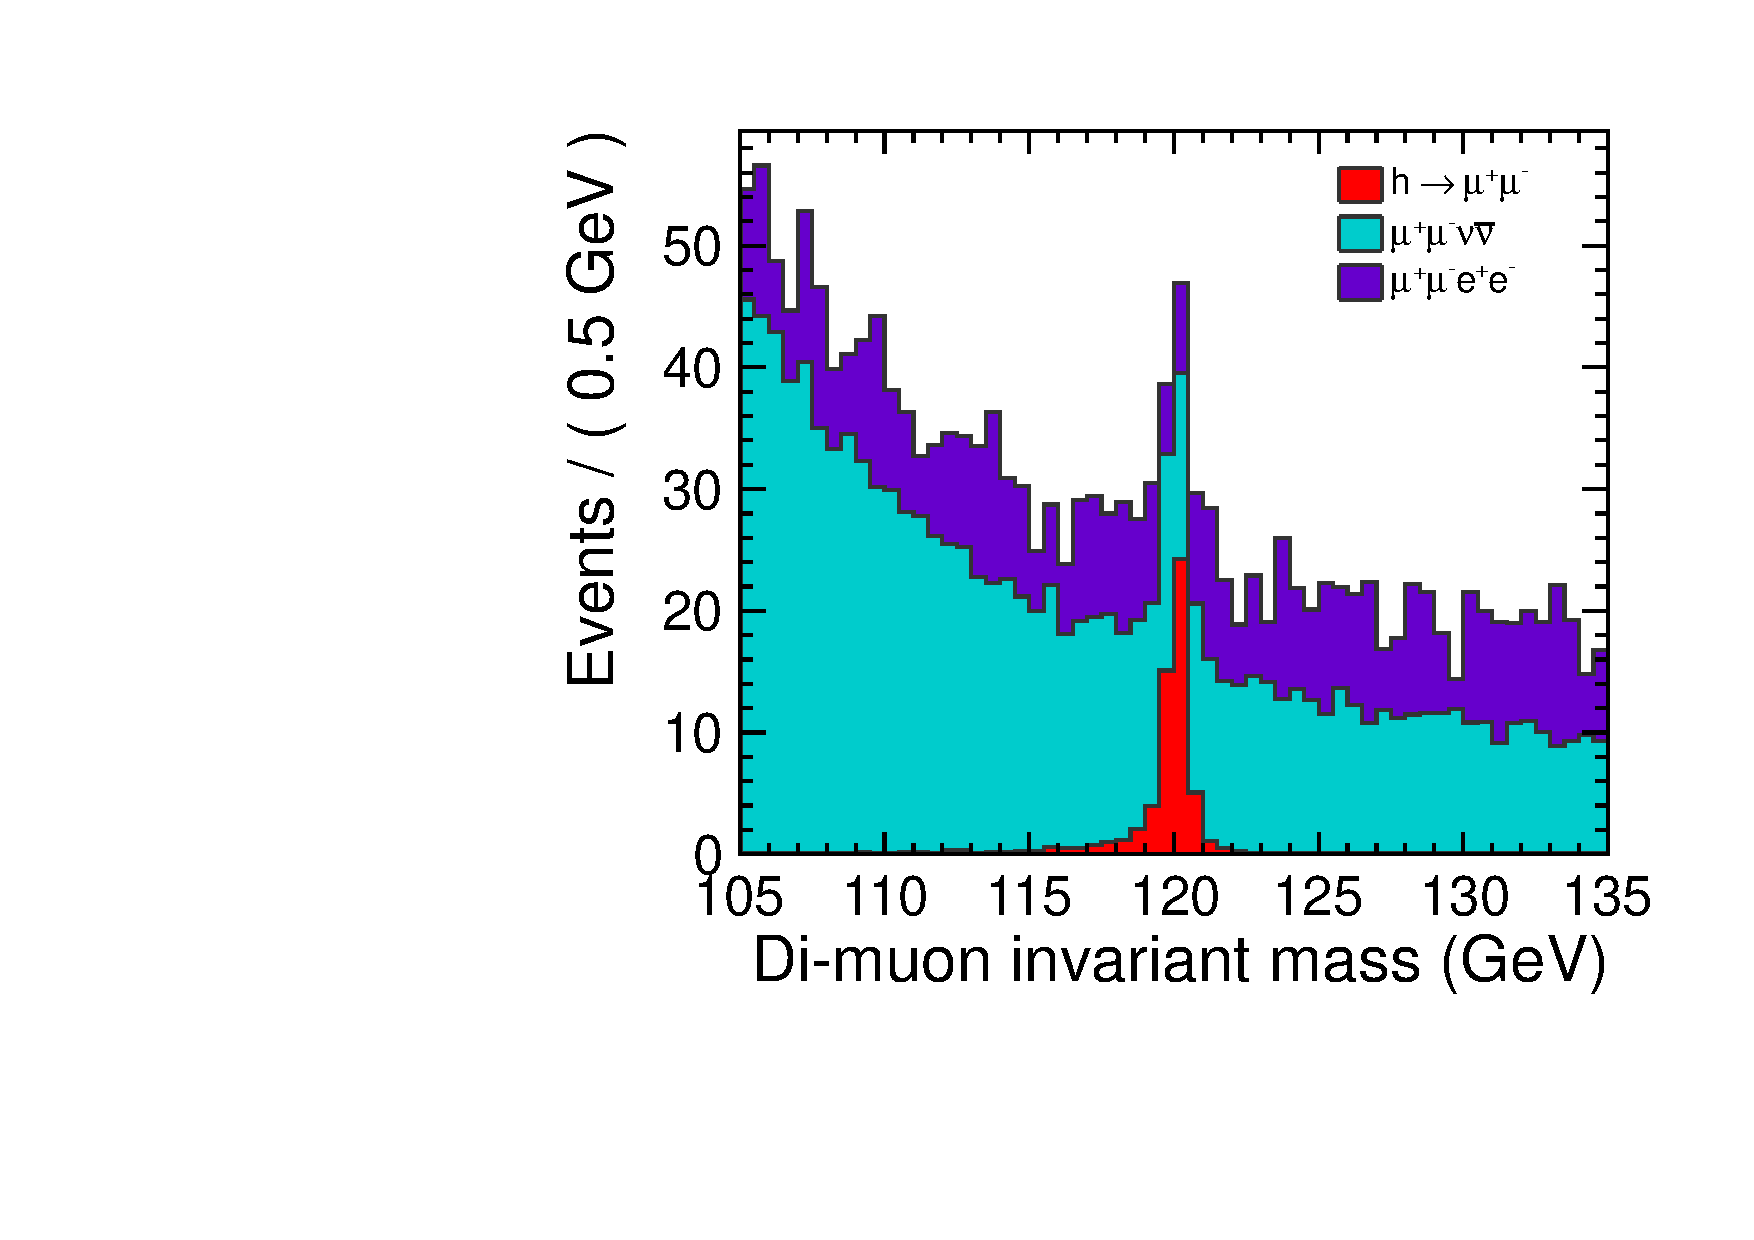
\includegraphics[width=5cm]{ee_h_mumu_mass_mh120GeV}
\column{6cm}
\centering
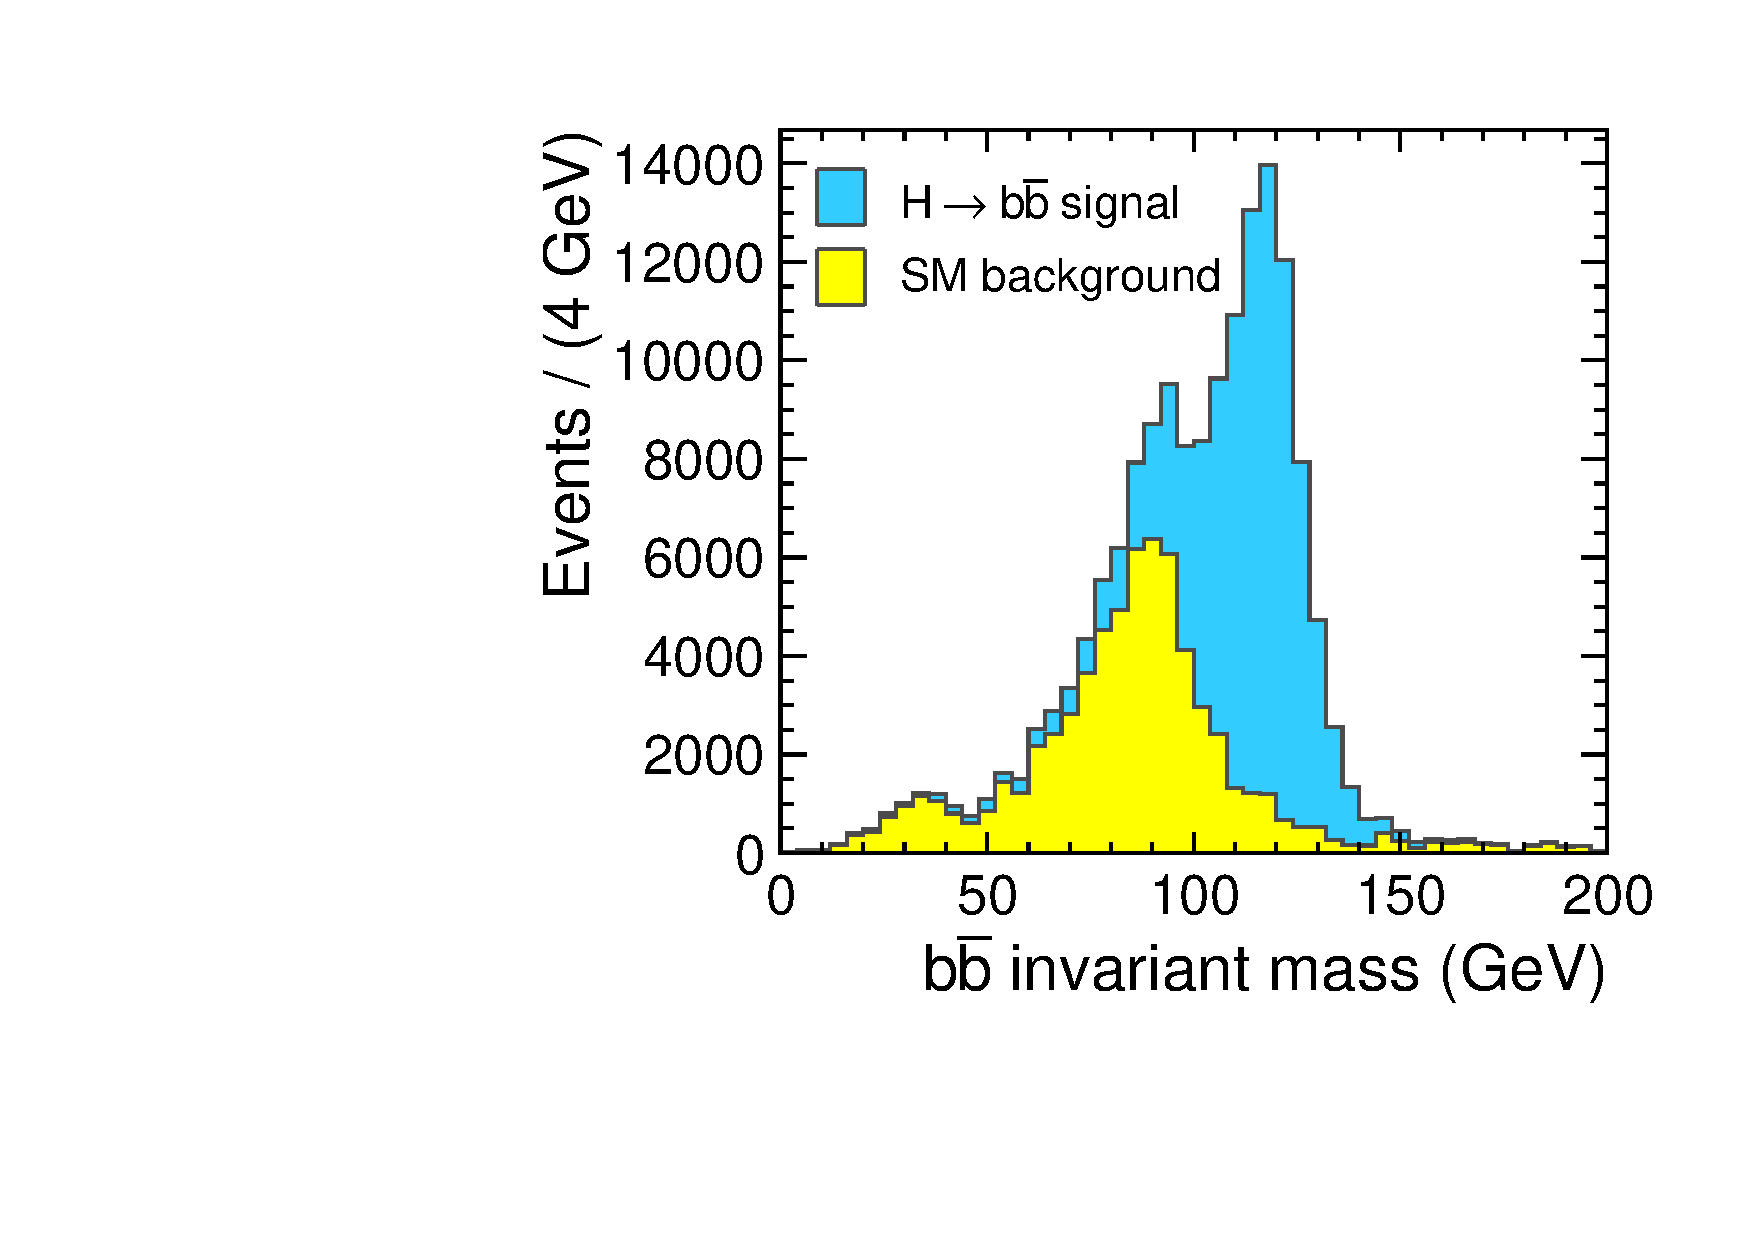
\includegraphics[width=5cm]{ee_h_bb_mass_mh120GeV}
\end{columns}
\end{frame}

\begin{frame}
\frametitle{Super Symmetry}
2 models considered to test several detector aspects: b-tagging, PFA, etc.
\begin{columns}[c]
\column{6cm}
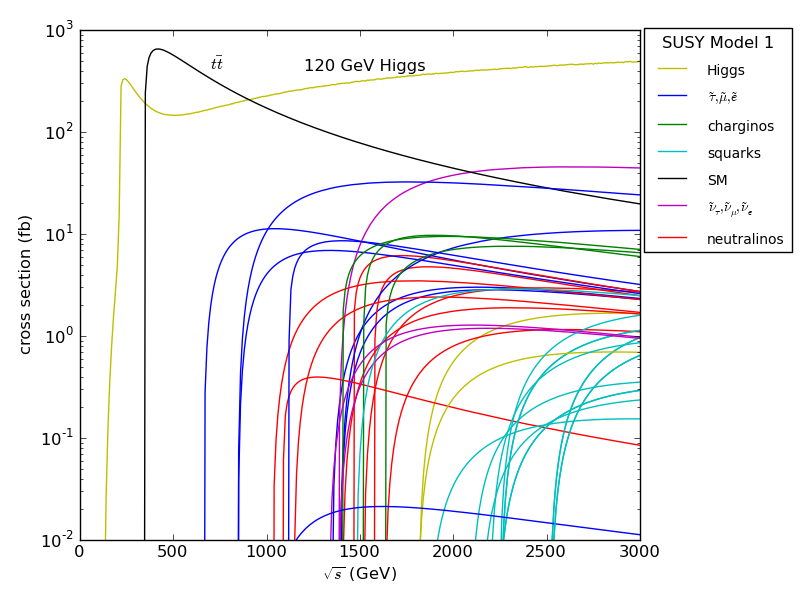
\includegraphics[width=6cm]{susy_model1.png}
\column{6cm}
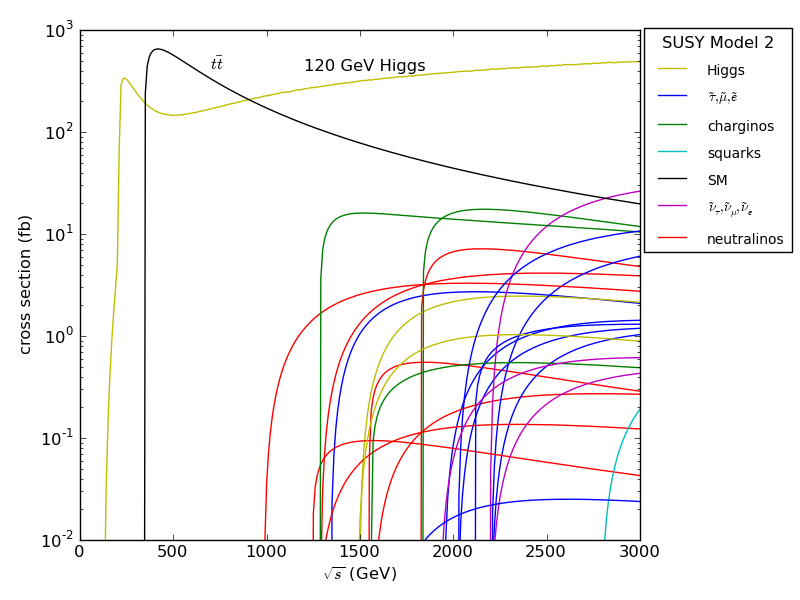
\includegraphics[width=6cm]{susy_model2.png}
\end{columns}
\begin{itemize}
  \item High Scale structure of the theory
  \item Test of Neutralino Dark Matter Hypothesis
\end{itemize}
\end{frame}

\begin{frame}
\frametitle{New physics scenarii}
% \begin{itemize}
%   \item Higgs strong interactions
%   \item Z'
%   \item Contact interactions
%   \item Extra dimensions
% \end{itemize}
\begin{center}
{\scriptsize
 \begin{tabular}{ ccccc }
    \toprule
 New particle &     LHC14 & SLHC & LC800 & CLIC3\\
 Luminosity & $100\textrm{fb}^{-1}$ & $1\textrm{ab}^{-1}$&
 $500\textrm{fb}^{-1}$& $1\textrm{ab}^{-1}$\\
\midrule
squarks [TeV] &   2.5 & 3 & 0.4 & 1.5 \\
sleptons [TeV] &   0.3 & - & 0.4 & 1.5 \\ 
$\textrm{Z}'$ ({\tiny SM ~couplings}) [TeV]  &  5 & 7 & 8 & 20   \\ 
%\Zprime ({\tiny SM~couplings})  &     5& 6  & 8 & 22 \\
%$q*$      &    6.5 & 7.5 & 0.8 & 3 \\
%$l*$       &   3.4 & - & 0.8 & 3 \\
2 extra dims $M_D$ [TeV]  &    9 & 12 & 5-8.5 & 20-30 \\
%$W_L W_L$      &  3.4sig& >3.4sig& -& 70sig\\
TGC (95\%)  ({\tiny \rm $\lambda_{\gamma} $~coupling}) &   0.001& 0.0006& 0.0004& 0.0001 \\
$\mu$ contact scale [TeV] &  15& - & 20 & 60 \\
Higgs compos. scale [TeV] & 5-7 & 9-12 & 30 & 30\\
    \bottomrule
  \end{tabular}
  }
 \end{center}
\end{frame}

\section[CLIC]{A few words on the CLIC machine and beam} 
\begin{frame}
\frametitle{The CLIC accelerator}
\begin{columns}[c]
\column{6cm}
\begin{itemize}
  \item Based on 2 beams, normal conducting accelerator
  \item 3TeV nominal 
  \item Luminosity spectrum: 30\% of the events in peak 1\% of the energy
  distribution
  \item Full luminosity: $5.4\times
  10^{34}\textrm{cm}^{-2}\,\textrm{s}^{-1}$
\end{itemize}
\column{6cm}
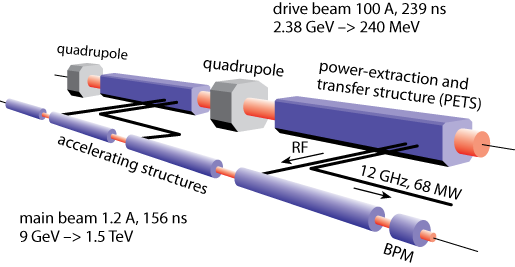
\includegraphics[width=6cm]{accel}
\end{columns}
\end{frame}

\begin{frame}
\frametitle{A particular beam structure}
\begin{itemize}
  \item CLIC: trains at 50Hz, 1 train is 312 bunches, 0.5ns apart
  \item ILC: trains at 5Hz, 1 train is 1300 bunches, 700ns apart
\end{itemize}
\centering
\begin{tabular}{lccc}
 & LEP2 & ILC 0.5TeV & CLIC 3TeV\\
 \hline
L [$\textrm{cm}^{-2}\,\textrm{s}^{-1}$] & $5\times 10^{31}$ & $2\times 10^{34}$& $5.4\times 10^{34}$ \\ 
\hline
Crossing angle & ~ & 14mrad & 20mrad\\
\hline
BX separation & 22$\mu$s & 700ns & \alert{0.5ns}\\
\hline
Nb $\gamma\gamma\to\textrm{had}$/BX & negligible & 0.2 & \alert{3.2}\\
\hline
Nb incoherant pairs/BX & negligible & $1\times 10^5$ & \alert{$3\times10^5$}\\
\hline
\end{tabular}
~\\
~\\
\alert{Very large machine induced background rate!}
\end{frame}

%\begin{frame}
%\frametitle{Running conditions}
%overlay, pairs
%\end{frame}

\section{The detectors}
\begin{frame}
\frametitle{The detector requirements}
\begin{itemize}
  \item High resolution pixel detector for displaced vertices identification:\\
  {\scriptsize
  \begin{tabular}{lc}
  p = 1 Gev & $\sigma_{d0}\sim20\mu m$\\
  p = 100 GeV & $\sigma_{d0}\sim5\mu m$
  \end{tabular}
  }~\\ ~\\
  \item Momentum resolution:\\
  {\scriptsize 
  \begin{tabular}{lc}
   p = 1 Gev & $\sigma(p_{\textrm{T}})/p_{\textrm{T}}=0.1\%$\\
   p = 100 Gev & $\sigma(p_{\textrm{T}})/p_{\textrm{T}}=0.2\%$
  \end{tabular}
   }~\\ ~\\
  \item Good jet-energy resolution (W/Z separation)\\
  {\scriptsize 
  \begin{tabular}{lc}
  E= $10^2$ GeV & $\sigma(E_j)/E_j \sim4\%$\\
  E= $10^3$ GeV & $\sigma(E_j)/E_j \sim3.5\%$
  \end{tabular}
  }~\\ ~\\
  \item Trigger less readout of full train: time stamping, multi-hit capacity,
  filtering algorithms during reconstruction
\end{itemize}
\end{frame}
\begin{frame}
\frametitle{The CLIC detectors}
Main differences with ILC concepts:
\begin{itemize}
  \item Denser barrel HCAL, using tungsten, 7.5$\lambda$
  \item Redesign of the vertex and forward detectors to account for the higher
  rates
\end{itemize}
\begin{columns}[c]
\column{6cm}
\centering
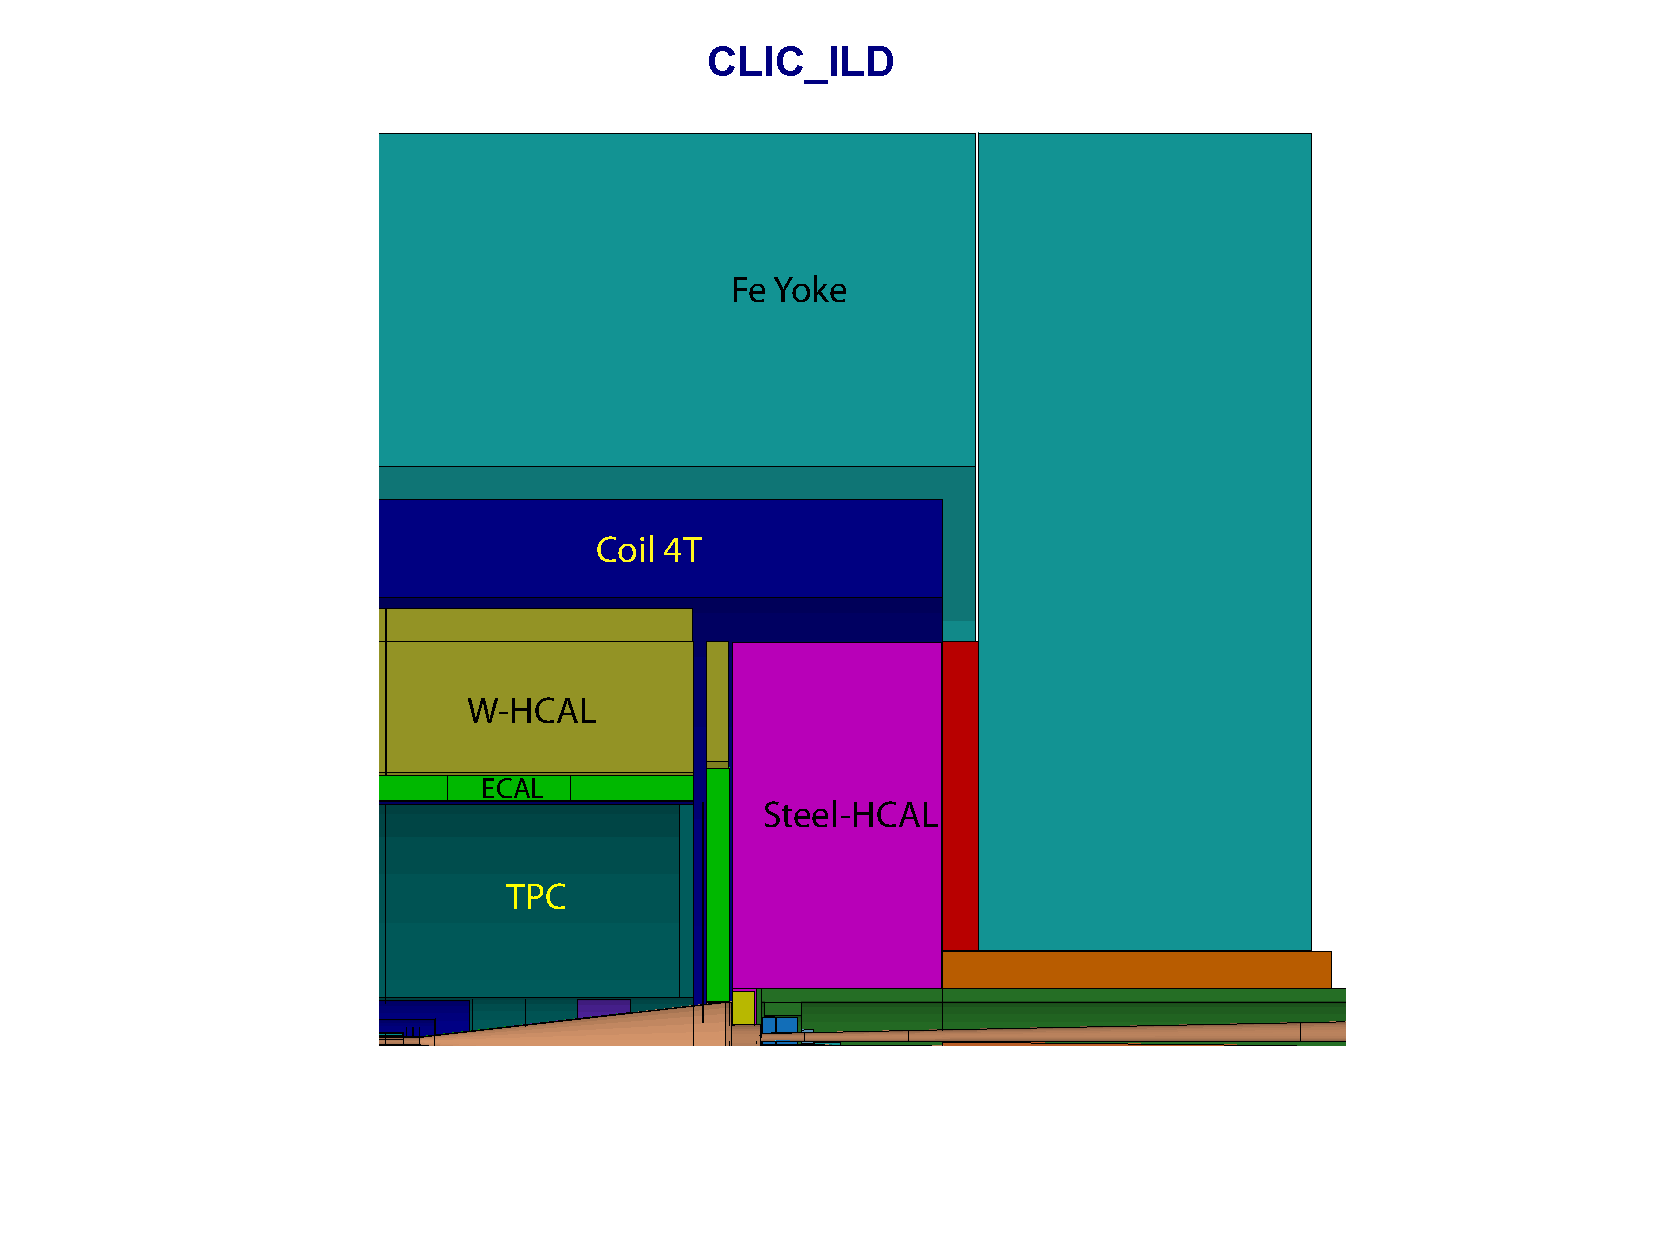
\includegraphics[width=5cm]{CLIC_ILD_xz_box_view1.pdf}
\column{6cm}
\centering
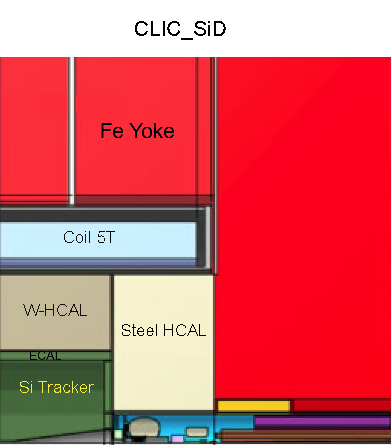
\includegraphics[width=4.5cm]{CLIC_SiD_xz_box_view.pdf}
\end{columns}
\end{frame}

\section[Bkg suppression]{Background suppression using timing}
\begin{frame}
\frametitle{Background suppression: use of timing resolution}
\begin{columns}[c]
\column{5cm}
\centering
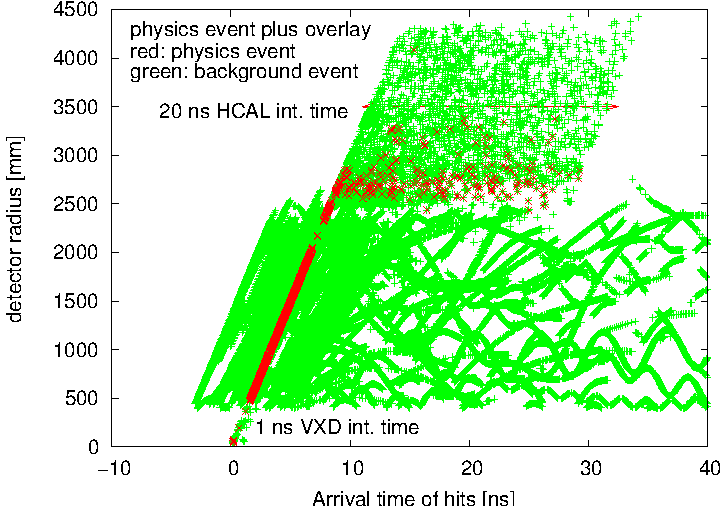
\includegraphics[width=5cm]{Overlayed}
\column{6cm}
{\scriptsize
\begin{tabular}{lcc}
Subdetector &Reco. window & hit resolution\\
ECAL &10 ns& 1 ns\\
HCAL Endcaps &10 ns &1 ns\\
HCAL Barrel &100 ns &1 ns\\
Silicon Detectors &10 ns &10/$\sqrt{12}$ ns\\
TPC &entire bunch train &n/a
\end{tabular}
}
\end{columns}
\begin{columns}[c]
\column{6cm}
\centering
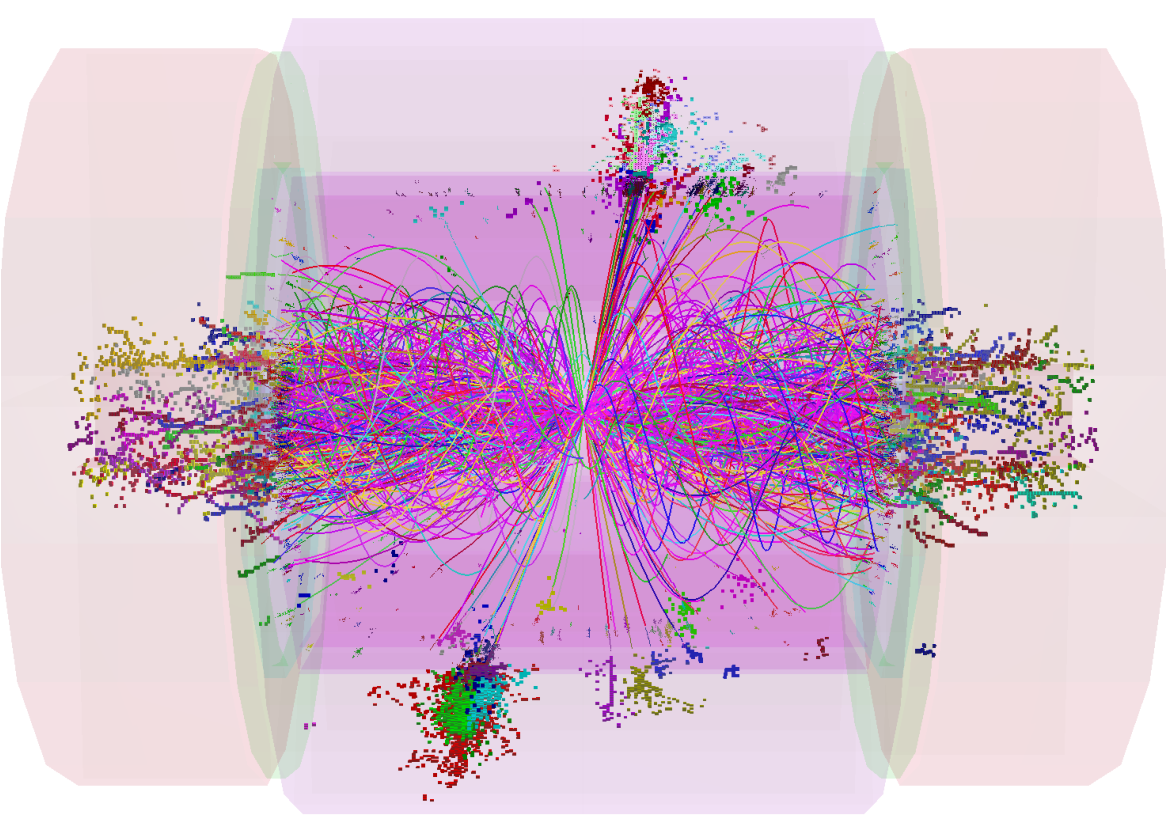
\includegraphics[width=4cm]{EventPictureNoPFOSelector.pdf}\\
No cuts
\column{6cm}
\centering
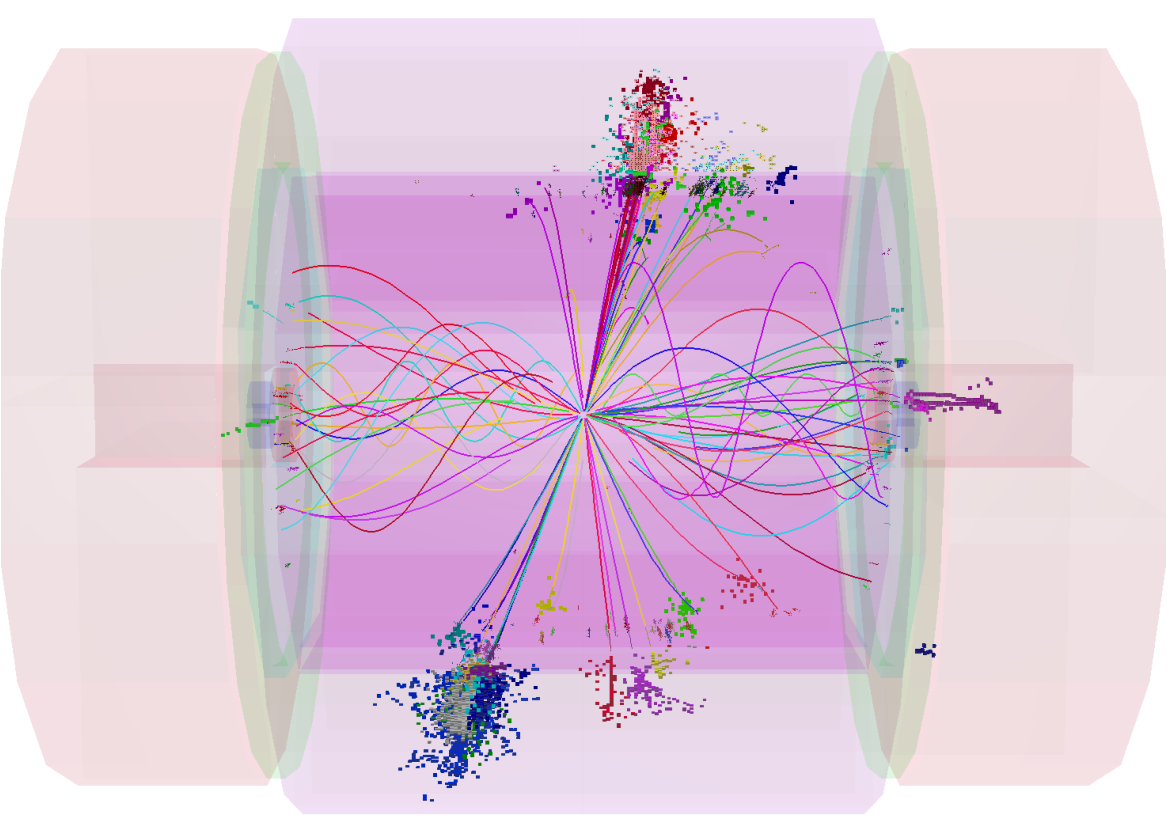
\includegraphics[width=4cm]{EventPicturePFOSelector.pdf}\\
Tight timing cuts
\end{columns}
\end{frame}

\section[Benchmarks]{The benchmark channels}
\begin{frame}
\frametitle{The benchmark channels}
6 benchmark channels to assess detector performance:
\begin{itemize}
\item $\Pep\Pem \to \Ph \Pgne \Pagne, \Ph \to \mu^+\mu^-, \Ph \to
\Pbottom\APbottom$,
\item  $\Pep\Pem \to \PHp \PHm$, $\Pep\Pem \to \PHz \PA$, 
\item $\Pep\Pem \to \PSq_R \PaSq_R$, 
\item $\Pep\Pem \to \PSl \PaSl \,(\ell = \Pe,\Pgm,\Pgne)$, 
\item $\Pep\Pem \to \PSgxpm_i \PSgxmp_j,\, \Pep\Pem \to \PSgxz_i \PSgxz_j$,
\item  $\Pep\Pem \to \Pqt \Paqt$ (500~GeV).
\end{itemize}
\end{frame}

\begin{frame}
\frametitle{SM Higgs decays}
\begin{columns}[c]
\column{6cm}
\centering
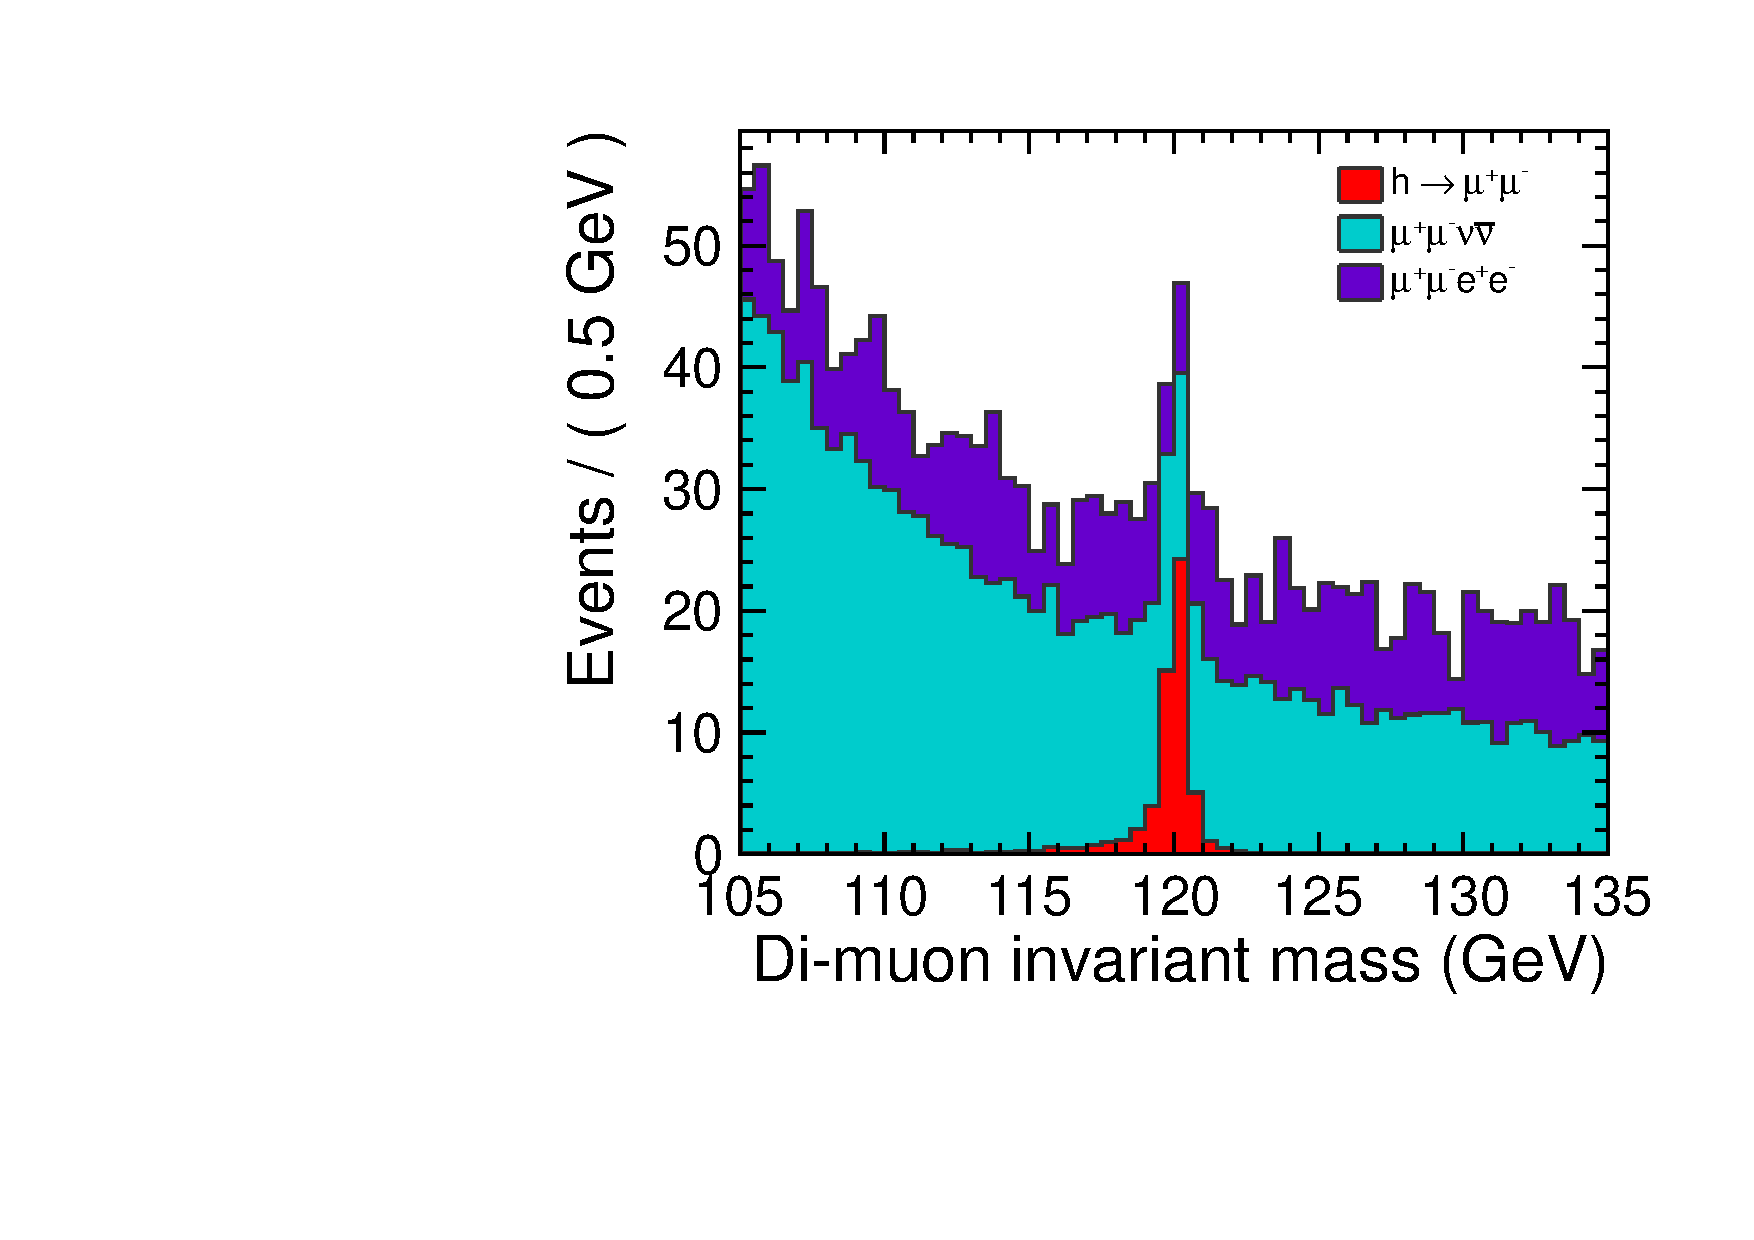
\includegraphics[width=5cm]{ee_h_mumu_mass_mh120GeV}
\column{6cm}
\centering
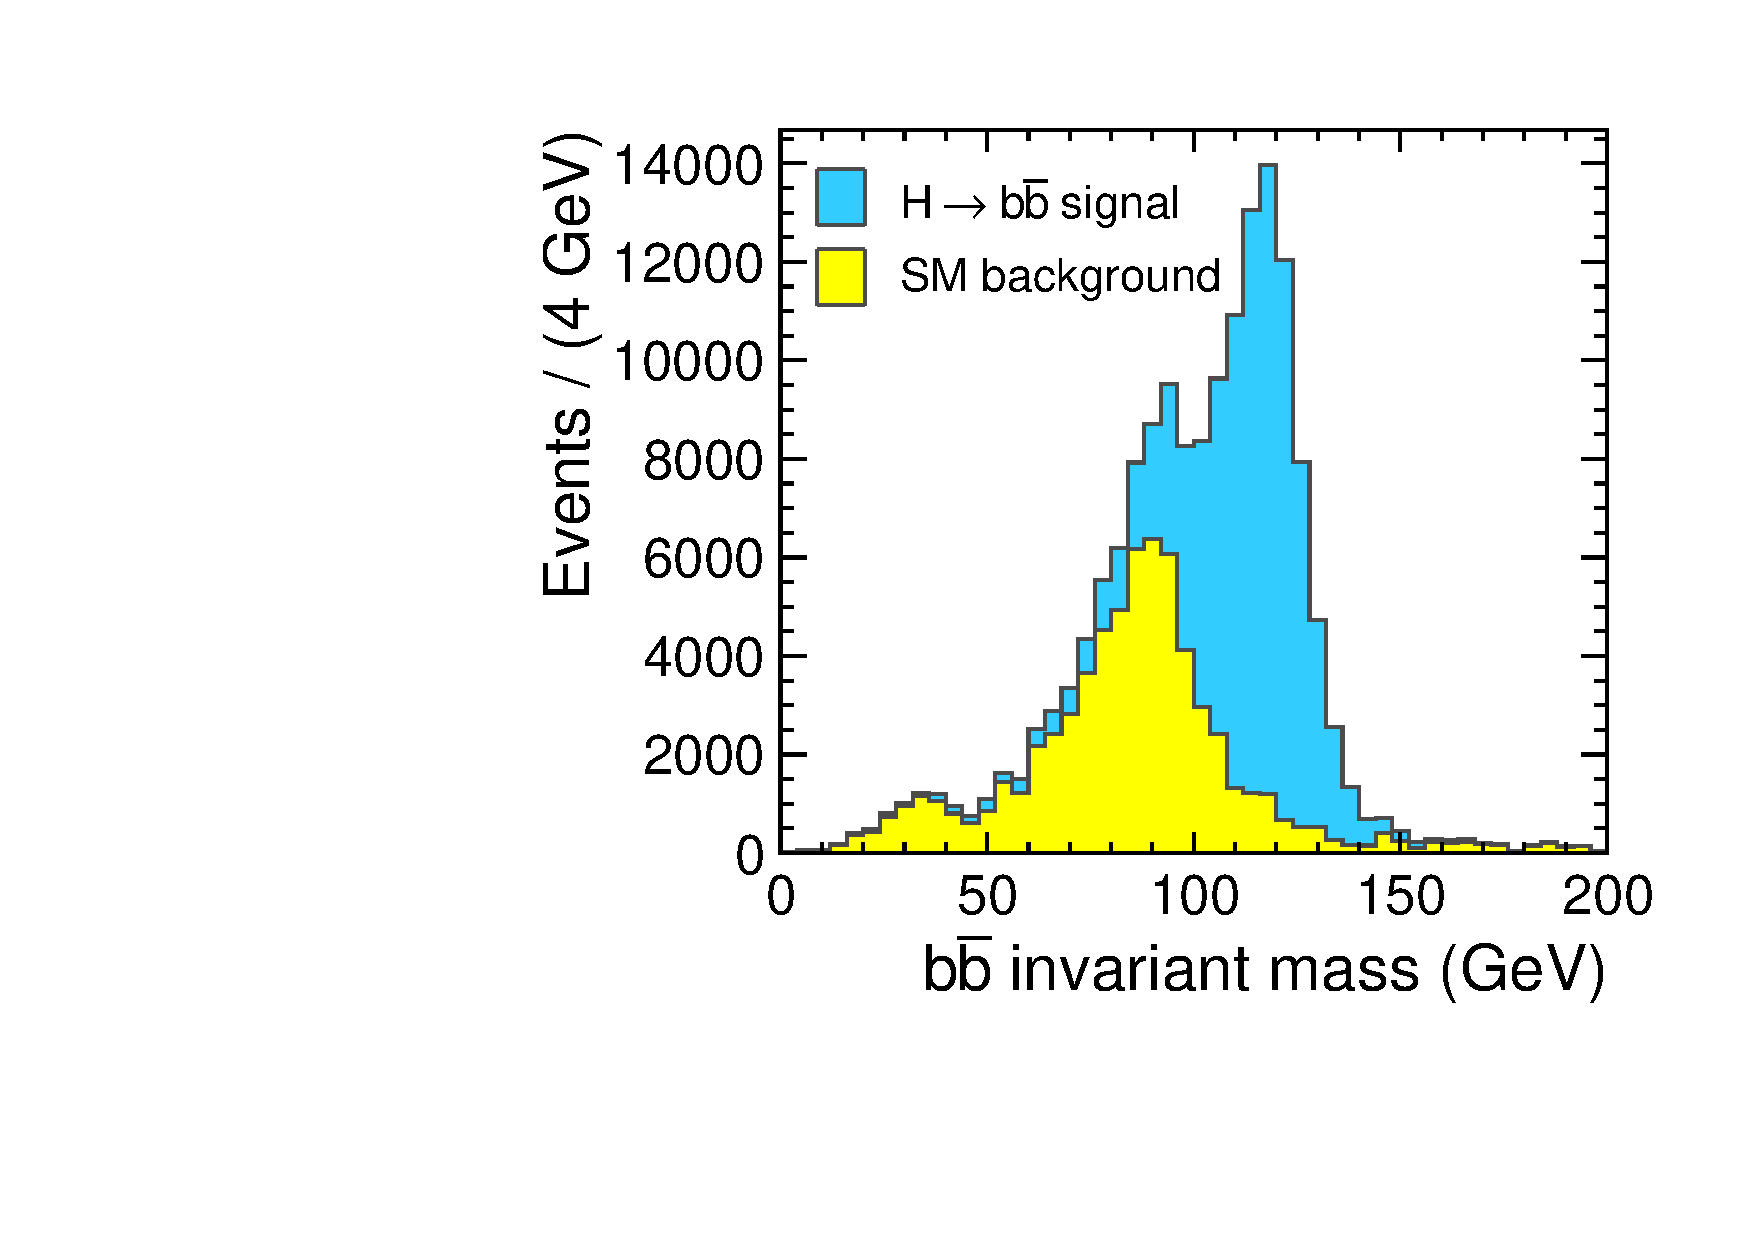
\includegraphics[width=5cm]{ee_h_bb_mass_mh120GeV}
\end{columns}
Cross section measurements:
\begin{itemize}
  \item
  $\sigma(\sigma_{\Ph\to\Pbottom\APbottom})/\sigma_{\Ph\to\Pbottom\APbottom} =
  0.22\%$ stat.
  \item $\sigma(\sigma_{\Ph\to\Pmuon\APmuon})/\sigma_{\Ph\to\Pmuon\APmuon}
  = 23\%$ stat.
\end{itemize}
$\Rightarrow$ Evaluation of b-tagging and momentum resolution
\end{frame}
\begin{frame}
\frametitle{Heavy Higgs: $\PH^0\PA\to\Pbottom\APbottom\Pbottom\APbottom$,
$\PH^+\PH^-\to\Ptop\APbottom\Pbottom\APtop$}
\centering
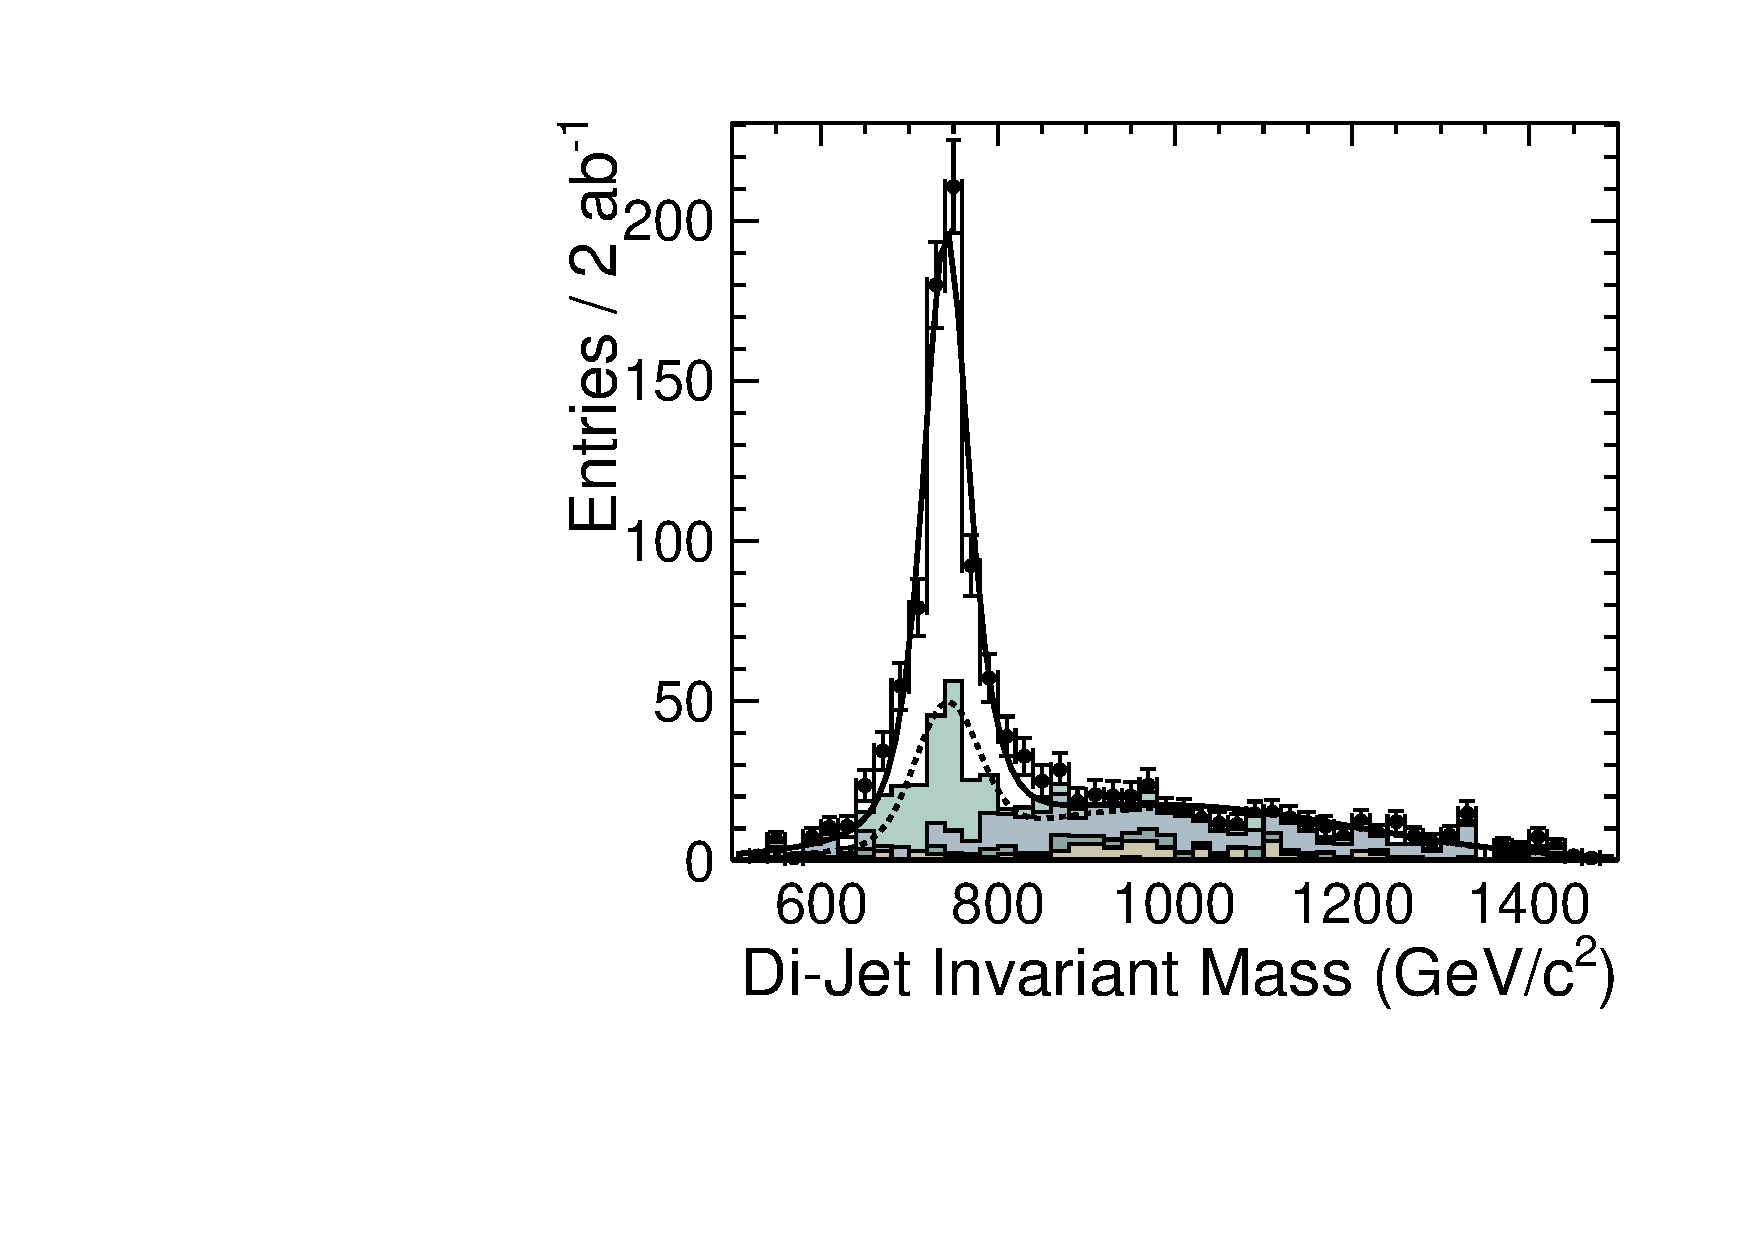
\includegraphics[width=4cm]{HAMass742_Bkg_CKFM_00BX_FJ.pdf}
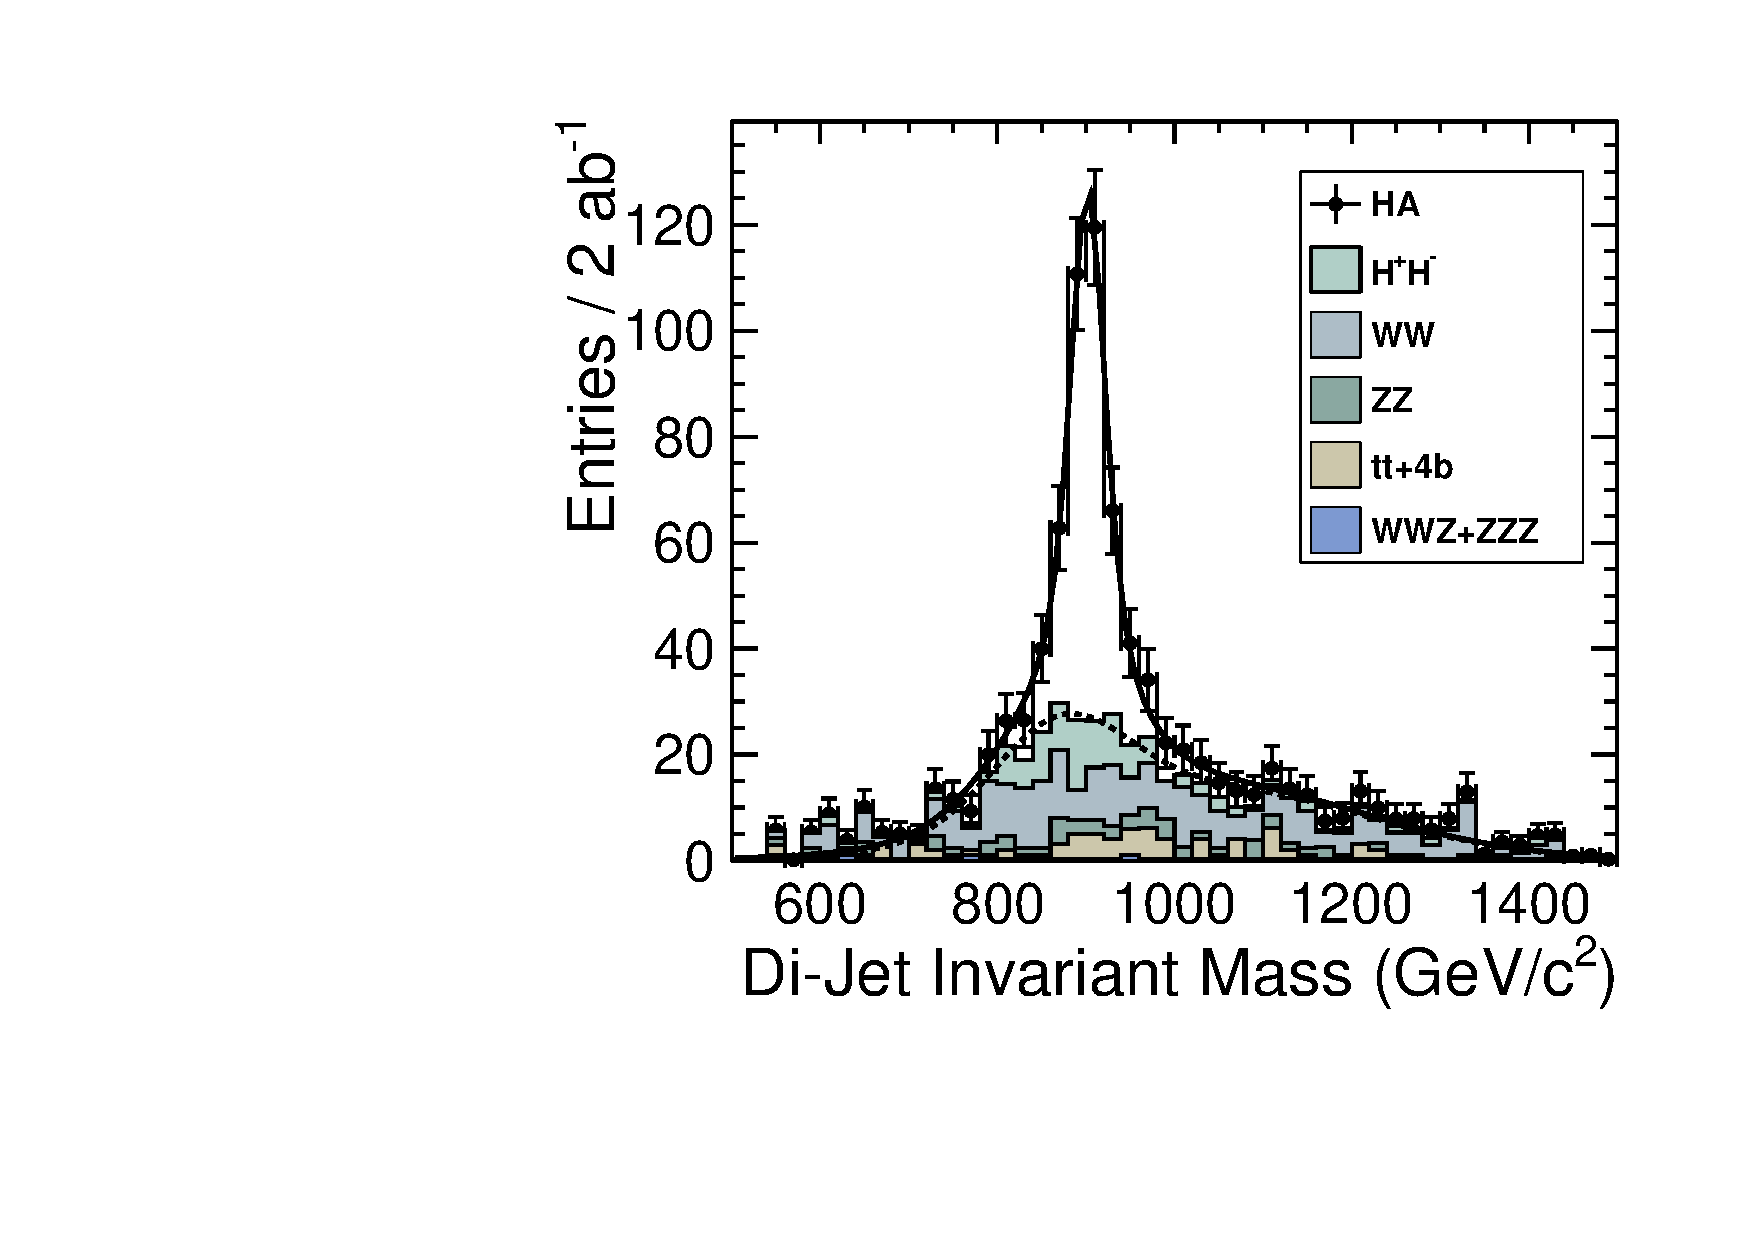
\includegraphics[width=4cm]{HAMass902_Bkg_CKFM_00BX_FJ.pdf}\\
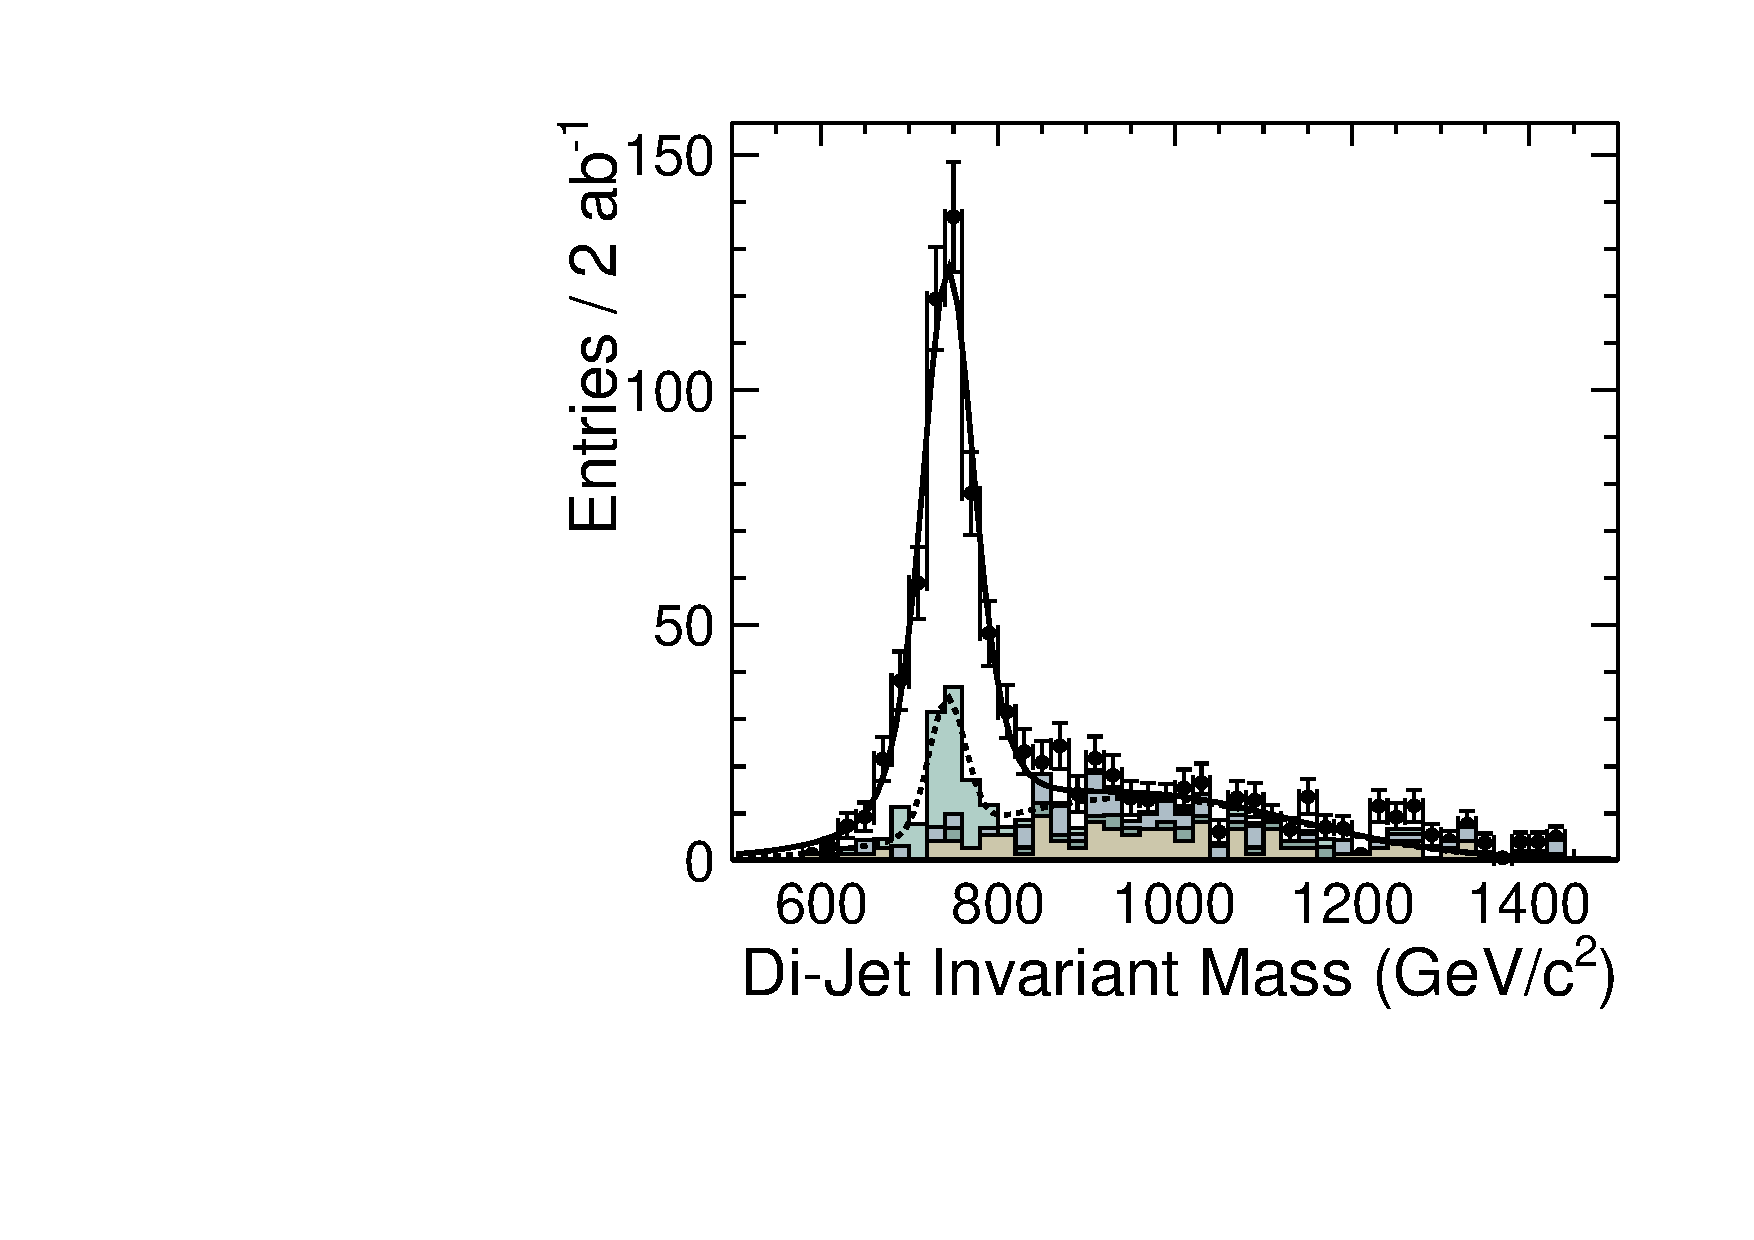
\includegraphics[width=4cm]{Hpm_Mass742_Bkg_CKFM_00BX_FJ.pdf}
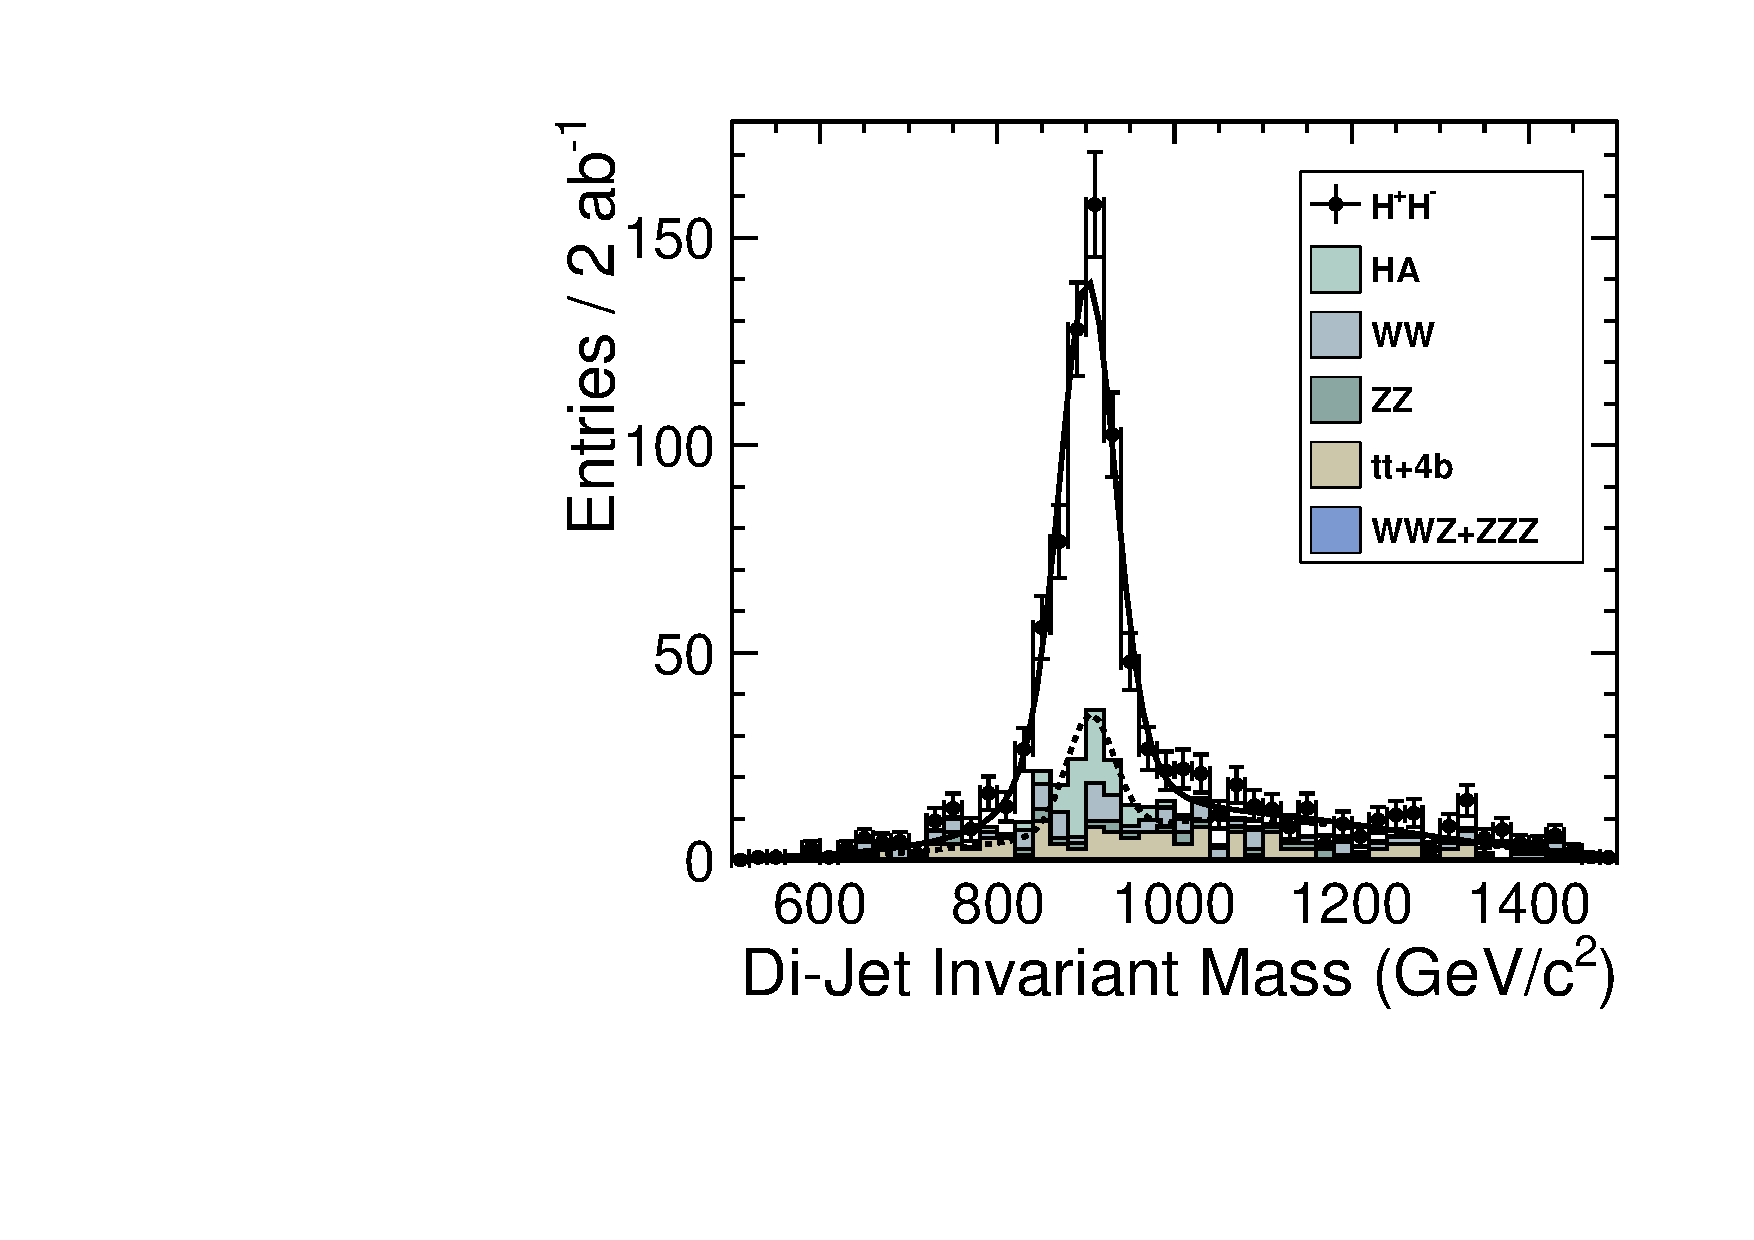
\includegraphics[width=4cm]{Hpm_Mass902_Bkg_CKFM_00BX_FJ.pdf}\\
{\scriptsize Statistical accuracy $\sigma(M)/M \sim0.3\%$.}\\
$\Rightarrow$ Evaluation of b-tagging and heavy jet reconstruction
\end{frame}
\begin{frame}
\frametitle{Squarks and Sleptons}
\begin{columns}[c]
\column{6cm}
\centering
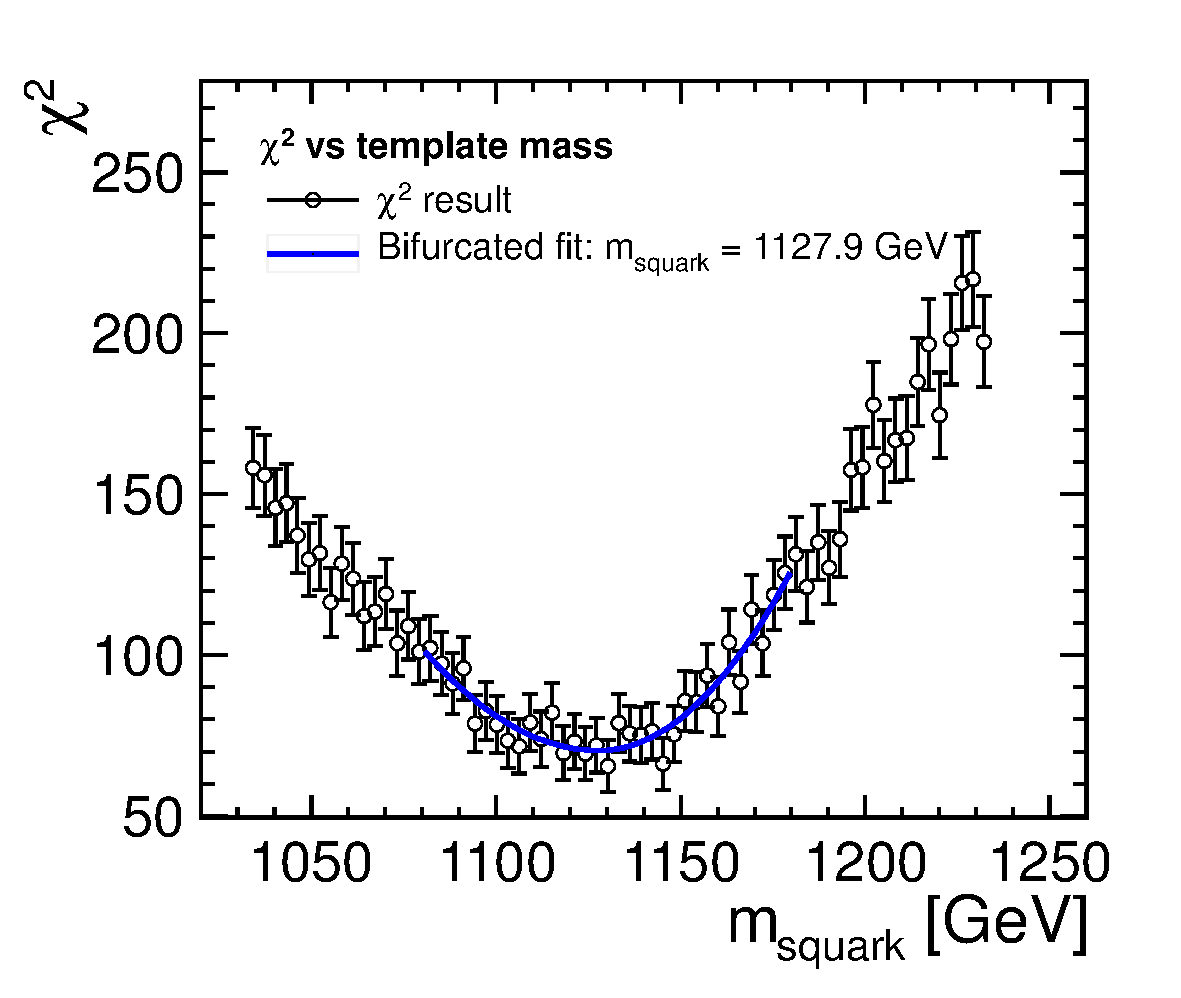
\includegraphics[width=5cm]{TemplateFit_Chi2SquarkMass.pdf}\\
\column{6cm}
\centering
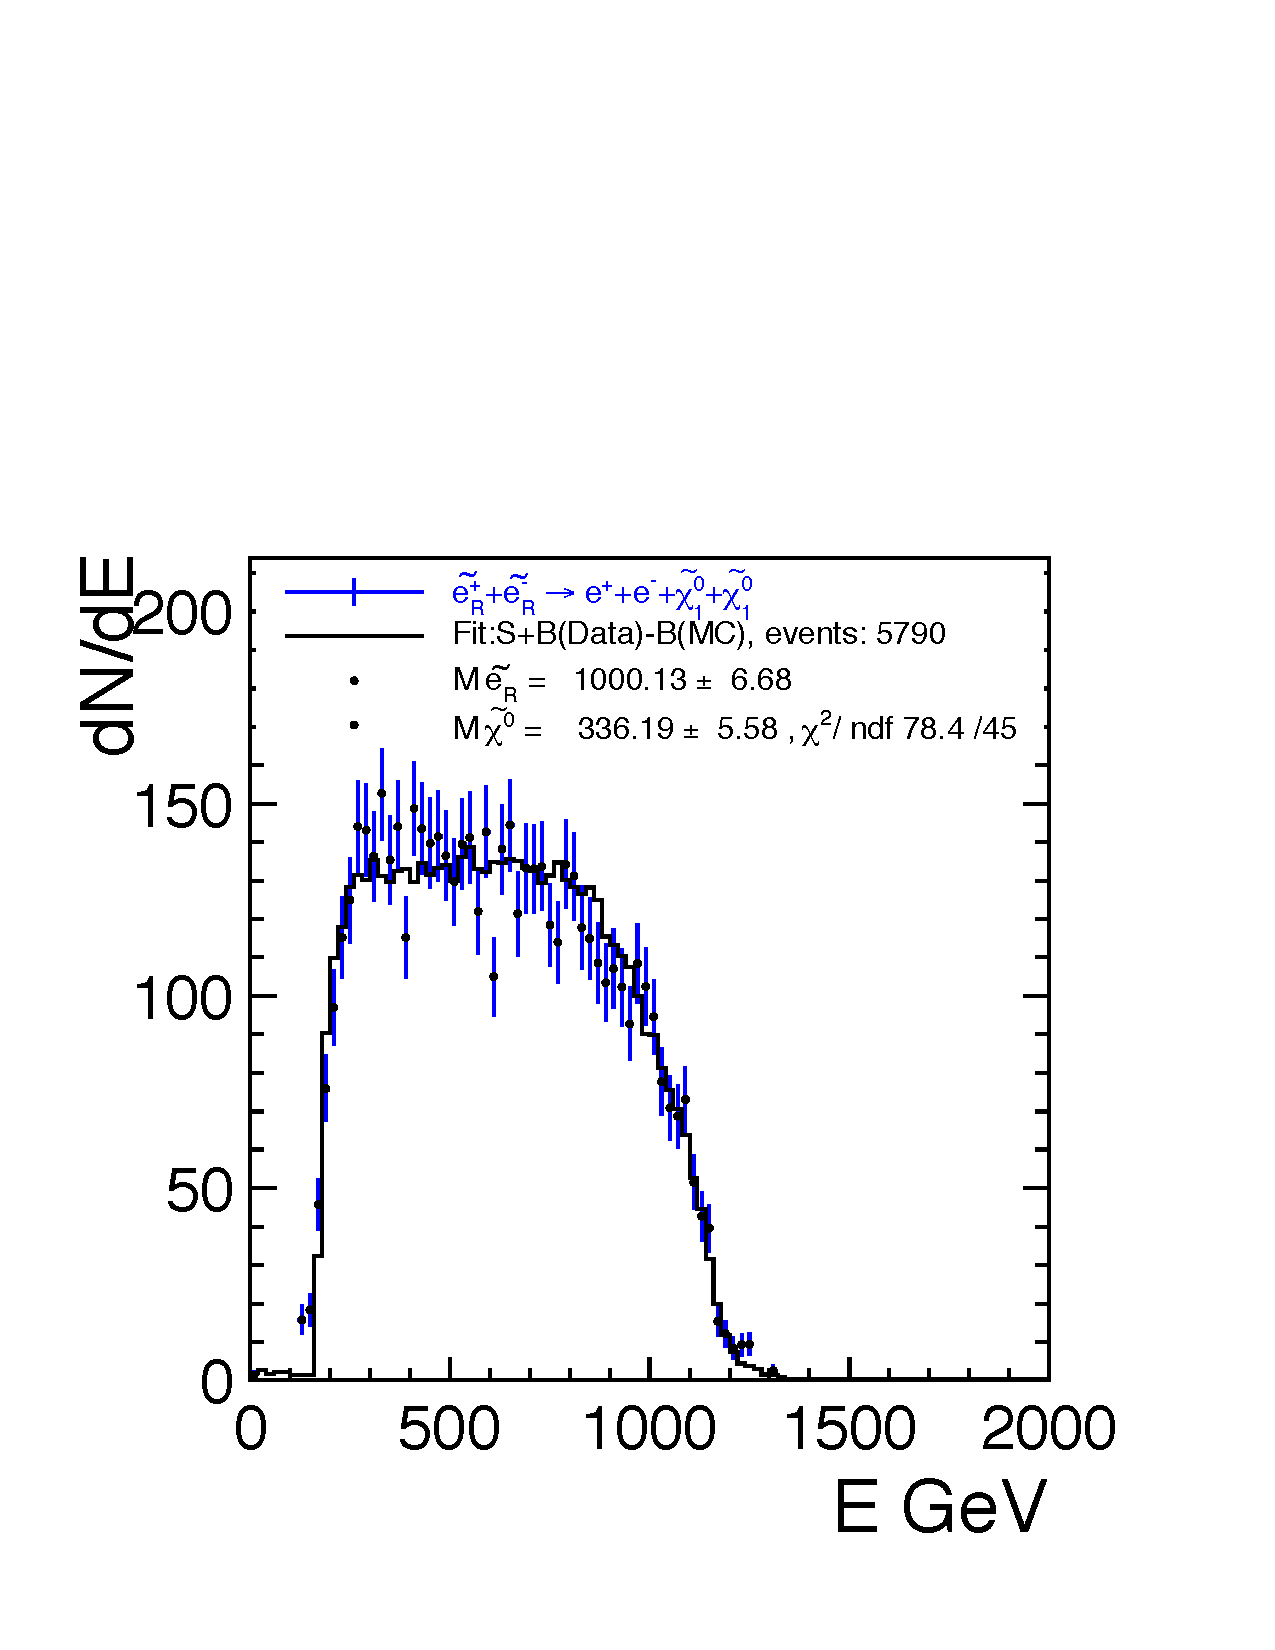
\includegraphics[width=5cm]{202_H1LPADC4.pdf}
\end{columns}
\begin{columns}[c]
\column{6cm}
\centering
$\sigma(m_{\PSq_{R}})/m_{\PSq_{R}}=0.5\%$
\column{6cm}
\centering
$\sigma(m_{\PSgm_{R}})/m_{\PSgm_{R}} = 0.6\%$\\
$\sigma(m_{\PSe_{R}})/m_{\PSe_{R}} = 0.3\%$\\
$\sigma(m_{\PSgxzi})/m_{\PSgxzi} = 1-2\%$
\end{columns}
~\\
$\Rightarrow$ Tests of jet reconstruction and Particle ID
\end{frame}
\begin{frame}
\frametitle{Gauginos}
\centering
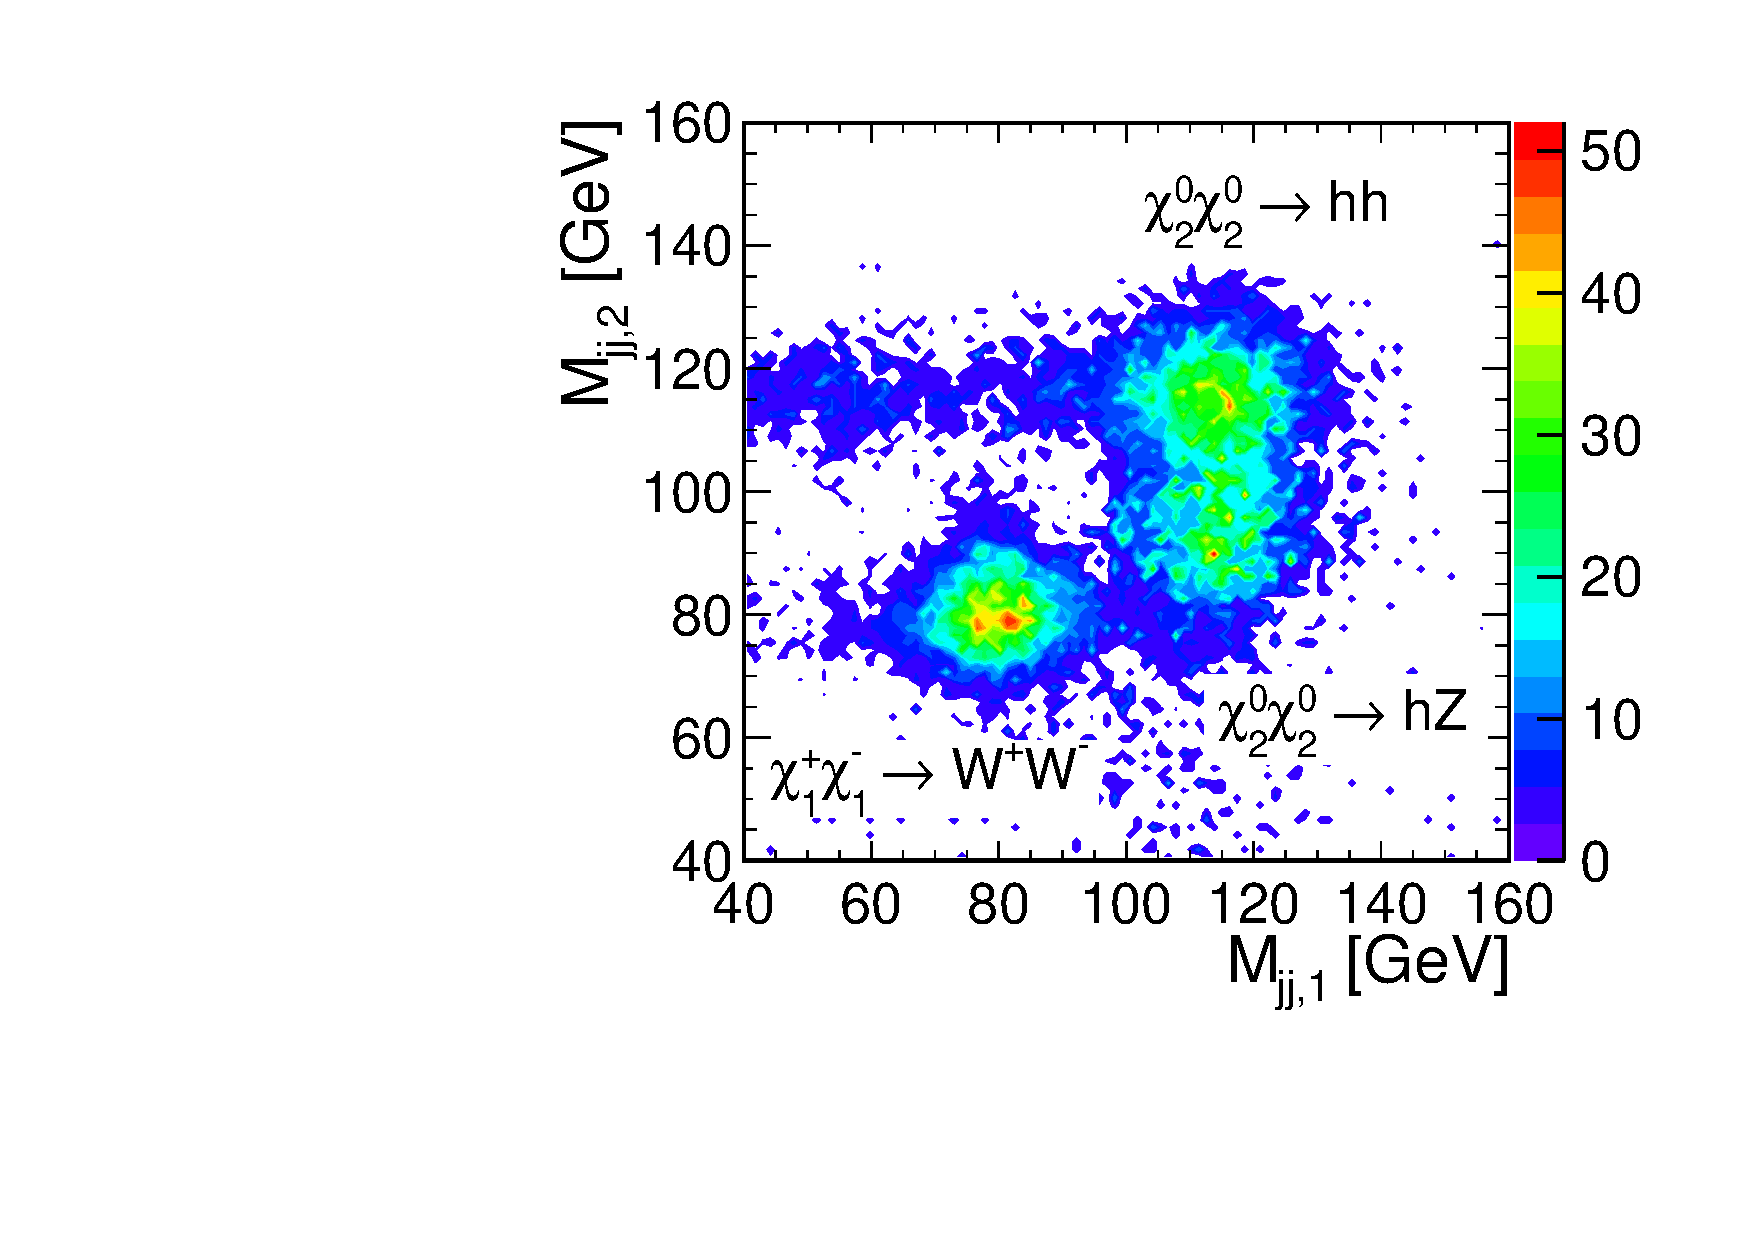
\includegraphics[width=6cm]{../WhizardWorkshop/MassPlot2D}\\
{\scriptsize 
\begin{tabular}{c c c c}
       \toprule
       Parameter 1                & Uncertainty &          Parameter 2 & Uncertainty \\
       \midrule
       $M(\tilde{\chi}_{1}^{\pm})$ & $6.3$~GeV & $\sigma(\tilde{\chi}_{1}^{+}\tilde{\chi}_{1}^{-})$  & $2.2$\% \\
       $M(\tilde{\chi}_{1}^{0})$   & $3.0$~GeV & $\sigma(\tilde{\chi}_{1}^{+}\tilde{\chi}_{1}^{-})$  & $1.8$\% \\
       $M(\tilde{\chi}_{2}^{0})$   & $7.3$~GeV & $\sigma(\tilde{\chi}_{2}^{0}\tilde{\chi}_{2}^{0})$  & $2.9$\% \\
\end{tabular}}\\
~\\
$\Rightarrow$ Evaluation of jet energy resolution
\end{frame}
\begin{frame}
\frametitle{Top physics at 500GeV}
\centering
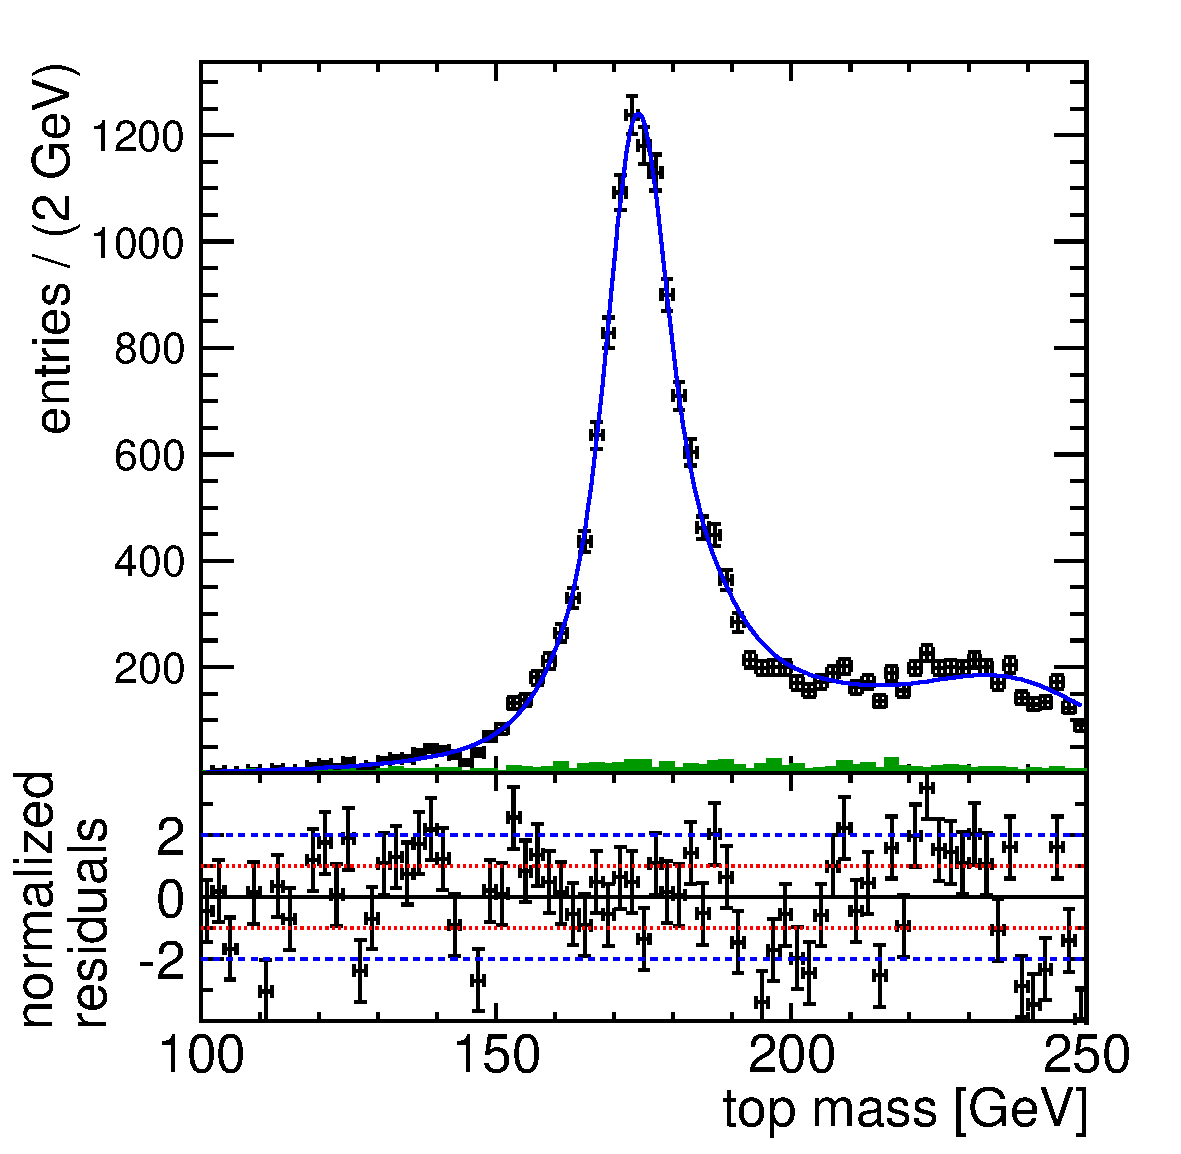
\includegraphics[width=5cm]{FinalFit-SemiLeptonic}
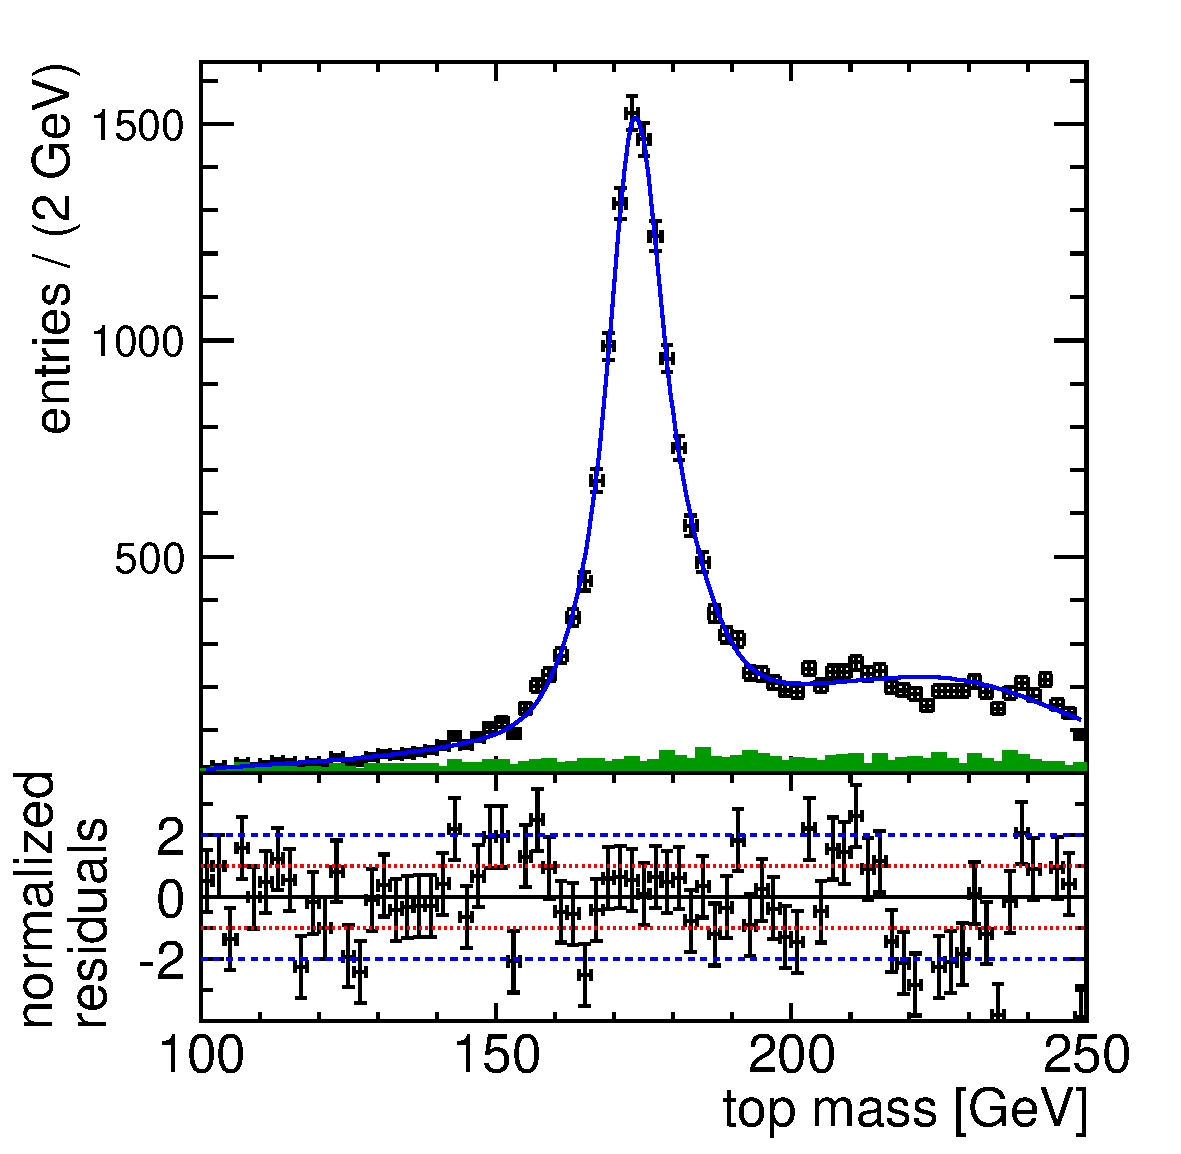
\includegraphics[width=5cm]{FinalFit-FullHadronic}\\
{\scriptsize
\begin{tabular}{l c c }
\toprule
 Top decay & Top mass (GeV) & Top width (GeV)\\
\midrule
                            Fully-hadronic & $174.07 \pm 0.08$ &  $1.33 \pm 0.22$\\
                            Semi-leptonic & $174.28 \pm 0.09$ &  $1.55 \pm 0.26$\\
\end{tabular}}\\
~\\
$\Rightarrow$ Compare with ILC
\end{frame}



\section[LCD for the DBD]{CERN LCD group in SiD DBD}
\begin{frame}
\frametitle{LCD group involvement in the SiD DBD}
\begin{itemize}
  \item $\Ptop\APtop\Ph$ analysis
  \item Production using ILCDIRAC
\end{itemize}
\end{frame}

\section{Conclusions}
\begin{frame}
\frametitle{Conclusions}

\begin{itemize}
  \item CDR is here:  \url{https://edms.cern.ch/document/1160419}
  \item Sign the CDR here:
  \url{https://indico.cern.ch/conferenceDisplay.py?confId=136364}
\end{itemize}
\end{frame}
\end{document}